% =====================================================================
%  C39 -- AAMAS 2027 main track (GTEP)
%
%  TRACK: GTEP, decided 2026-09-23 on three years of chairs'-report data plus
%  the novelty audit. COINE's stated scope (accountability, governance) reads
%  like the better fit, and the counter-argument is real -- Theorem 1 removes
%  the payment rule, after which no payment appears again. It loses to two
%  independent findings:
%    1. Base rates. Full-paper acceptance, 3-yr weighted: GTEP 31.3% vs COINE
%       19.0%. COINE is also tiny (N=122 over 3 years) and wildly unstable --
%       28% in 2023, 4% in 2024, 17% in 2025. GTEP sits at 29/30/35%.
%    2. Intellectual neighbourhood. The novelty audit found every nearest
%       prior work in economics -- Fadel-Segal (JET 2009), Kadan-Swinkels
%       (JET 2008), Georgiadis-Szentes (Econometrica 2020), Green-Laffont,
%       Holmstrom, FLM. None in a COINE venue. GTEP reviewers are the ones
%       equipped to judge this.
%  See docs/track_decision_2026-09-23.md for the full data and reasoning.
%
%  CLASS: AAMAS ships `aamas.cls`, which is `acmart` with an IFAAMAS
%  copyright modification. For submission replace the line below with
%      \documentclass[sigconf, anonymous]{aamas}
%  and drop `nonacm`. Formatting is otherwise identical, so the swap is a
%  one-line change and nothing in sections/ moves.
%
%  Limit: 8 pages excluding references. Double-blind. LaTeX mandatory.
%  Build: pdflatex main && bibtex main && pdflatex main && pdflatex main
% =====================================================================
\documentclass[sigconf, anonymous, nonacm]{acmart}

% acmart (and the AAMAS class derived from it) already loads amsmath and a font
% package that defines \Bbbk, so amssymb must be let in carefully.
\let\Bbbk\relax
\usepackage{amsmath,amssymb,amsthm}
\usepackage{booktabs}
\usepackage{tikz}
\usepackage{pgfplots}
\pgfplotsset{compat=1.18}

% acmart predefines most of these; only declare the ones that are missing, so
% the file works both standalone and under the conference class.
\makeatletter
\@ifundefined{theorem}{\newtheorem{theorem}{Theorem}}{}
\@ifundefined{lemma}{\newtheorem{lemma}[theorem]{Lemma}}{}
\@ifundefined{proposition}{\newtheorem{proposition}[theorem]{Proposition}}{}
\@ifundefined{corollary}{\newtheorem{corollary}[theorem]{Corollary}}{}
\theoremstyle{definition}
\@ifundefined{definition}{\newtheorem{definition}[theorem]{Definition}}{}
\@ifundefined{remark}{\newtheorem{remark}[theorem]{Remark}}{}
\makeatother

% --- the objects of the paper ---------------------------------------
\newcommand{\cube}{\{0,1\}^n}          % effort profiles
\newcommand{\Qn}{Q_n}                  % the n-cube as a graph
\newcommand{\gtwo}{\gamma_2}           % 2-domination number
\newcommand{\Kflat}{K_{\mathrm{flat}}} % flatness threshold
\newcommand{\Dopt}{D^\ast}             % constrained optimum
\newcommand{\Dnull}{D_0}               % unconstrained optimum
\newcommand{\Mn}{M_n}                  % E[min(|S|, n-|S|)]
\newcommand{\labels}{[K]}
\newcommand{\enc}{q}                   % stochastic encoder
\newcommand{\pay}{p}                   % bounded payment decoder
\newcommand{\rec}{\hat{s}}             % reconstruction decoder
\newcommand{\dH}{d_{\mathrm{H}}}       % Hamming distance
\newcommand{\TV}{\mathrm{TV}}
\newcommand{\simplex}{\Delta}
\newcommand{\dmin}{d_{\min}}
\providecommand{\E}{}\renewcommand{\E}{\mathbb{E}}
\providecommand{\Prob}{}\renewcommand{\Prob}{\mathbb{P}}
\providecommand{\R}{}\renewcommand{\R}{\mathbb{R}}
\newcommand{\ind}[1]{\mathbf{1}\{#1\}}
\newcommand{\sminus}{s_{-i}}
\DeclareMathOperator*{\argmin}{arg\,min}
\DeclareMathOperator*{\argmax}{arg\,max}


\begin{document}

\title{How Much Memory Does Accountability Cost?}
\subtitle{Exact Reconstruction--Incentive Frontiers for Compressed Multi-Agent Records}

\begin{abstract}
A record that must later settle payments and a record that must later be
read back are not the same object, and a size bound forces a choice between
them. We study that choice exactly. A record with $K$ labels must
(i)~permit reconstruction of a joint effort profile $S \in \cube$ with small
expected Hamming error, and (ii)~retain enough about each agent's unilateral
contribution that a \emph{bounded} payment computed from the record alone
rewards effort by at least $\gamma$, whatever the teammates did.

Our first result removes the payment rule from the problem: such a payment
exists for agent~$i$ if and only if every unilateral deviation by~$i$ moves the
retained label distribution by at least $\gamma$ in total variation, minimised
over mixtures of teammate behaviour. Accountability is exactly a lower bound on
the record's sensitivity to each individual, so a record whose margin falls below
an agent's effort cost cannot sustain that effort under any bounded payment rule
and any equilibrium concept---a constraint mechanism design must respect,
stated before a mechanism is chosen.

From it we obtain two exact results. The one-bit frontier is
$\Dopt(2,\gamma) = \Mn + n\gamma\bigl(\tfrac{n-1}{2} - \Mn\bigr)$, linear in
$\gamma$, for arbitrary bounded payments and arbitrary reconstruction. And for
\emph{every} full-support prior we characterise the threshold at which
accountability becomes free: it is the least $K$ admitting a prior-optimal
$K$-median code in which every non-centre has at least two centres at its own
nearest distance. Under the uniform prior this specialises to
$\Kflat(n) = \gtwo(\Qn)$, the $2$-domination number of the $n$-cube, giving
$\Kflat(7) = 32$ and $97 \le \Kflat(9) \le 128$ with machine-checkable
certificates. Escaping the tension costs about $85\%$ of per-agent resolution at
$n = 20$. Concrete compaction mechanisms land where the theory says: at $n=5$ two
records of the same size and the \emph{same} reconstruction error differ by
$1/2$ against $0$ in margin, so identical compression quality can be worth
everything or nothing for accountability.

\end{abstract}

\keywords{accountability; credit assignment; deferred settlement; bounded
payments; information-theoretic limits; domination number}

\maketitle

\section{Introduction}
\label{sec:intro}

A principal must pay $n$ agents for work already done, using only what was
written down. Between the work and the payment, the record was compressed: it
now distinguishes $K$ outcomes rather than $2^n$. Two questions are asked of
that record, and they are not the same question. \emph{Reconstruction} asks what
the team did, and is answered well by a record that merges profiles which are
cheap to confuse. \emph{Accountability} asks what each agent did, and is answered
only by a record that each agent, acting alone, visibly moves. A fixed budget $K$
cannot in general serve both. This paper computes the tradeoff exactly---where it
binds, how steep it is, and where it vanishes.

The object is a constraint on mechanism design rather than a mechanism. We show
that a record admits a bounded payment rewarding agent~$i$'s effort by $\gamma$
if and only if $i$'s unilateral deviation moves the record's label distribution
by $\gamma$ in total variation. So a record whose margin is below an agent's
effort cost cannot sustain that effort \emph{under any bounded payment rule and
any equilibrium concept}. That bound is fixed before a designer chooses anything,
and the rest of the paper computes what a budget buys.

\paragraph{Two contrasts that place the question.}
In Holmstr\"om's moral hazard in teams~\cite{holmstrom1982}, joint output hides
individual effort and no budget-balanced sharing rule makes effort a best
response. There, the per-agent signal \emph{never existed}: the production
technology did not produce one. Here it existed and a budget destroyed it, and
the question is how much of it must survive. Holmstr\"om relaxes budget balance
to restore incentives; we hold the payment bounded and ask what the \emph{record}
must retain.

The second contrast fixes the direction of the constraint. Differential privacy
and its relatives bound a record's sensitivity to any one individual from
\emph{above} and ask how much utility survives; we bound it from \emph{below} and
ask how much compression survives. The two are not dual---one is a privacy
guarantee, the other an accountability requirement---but the contrast locates the
object precisely: we ask for the least sensitivity a record must keep, not the
most it may have. Section~\ref{sec:related} returns to both.

\paragraph{Why the budget is not hypothetical.}
In contemporary multi-agent systems a coordinator that fans work out to
sub-agents does not keep what they did: each sub-agent runs in its own context
and returns a summary, and when the coordinator's own context fills, older
exchanges---including whatever it retained about its sub-agents---are replaced by
a summary of themselves. The binding constraint is a fixed context window, which
unlike a storage bill cannot be paid off, and sampling is unavailable because one
cannot discard $99.9\%$ of the episode currently running. Whatever survives is
then the only evidence for any later question about who contributed. Settling
from a merged record is already a live failure mode: in
Bittensor~\cite{bittensorweightcopier} validators submit weight vectors that
consensus merges, and dividends track agreement with the merged result, so a
validator that evaluates nothing and copies the stake-weighted average is
indistinguishable in the record from one that worked---and reportedly earns
more~\cite{bittensorfreeriding}. The deployed remedy changed the \emph{record},
encrypting weights until stale~\cite{bittensorcommitreveal}. We cite this as
evidence that settling from a merged record destroys unilateral sensitivity in
practice, and as nothing more: its binding constraint is temporal, not a bound on
record size.

\paragraph{Contributions.}
\begin{enumerate}
\item \textbf{Payment-decoder elimination} (Theorem~\ref{thm:elim}). A minimax
      argument removes the payment rule, leaving a condition on the record alone:
      every unilateral deviation must move the label distribution by at least
      $\gamma$ in total variation. Corollary~\ref{cor:effort} states the
      consequence as a bound mechanism design must respect.
\item \textbf{The exact one-bit frontier} (Theorem~\ref{thm:onebit}):
      $\Dopt(2,\gamma) = \Mn + n\gamma(\frac{n-1}{2} - \Mn)$ for
      $0 \le \gamma \le 1/n$, for arbitrary bounded payments and arbitrary
      reconstruction.
\item \textbf{The flatness threshold, for every full-support prior}
      (Theorem~\ref{thm:prior}). Accountability becomes free exactly at the least
      $K$ admitting a prior-optimal $K$-median code in which every non-centre has
      at least two centres at its own nearest distance, and an explicit record
      attains it.
\item \textbf{The uniform case is a graph invariant}
      (Corollary~\ref{cor:uniform}): $\Kflat(n) = \gtwo(\Qn)$, the
      $2$-domination number of the $n$-cube, with margin
      $1 - 1/\dmin \ge 1/2$. Evaluating it gives $\Kflat(3)=4$, $\Kflat(5)=10$,
      $\Kflat(7)=32$, $97 \le \Kflat(9) \le 128$, each with a certificate. The
      invariant is classical and we claim no novelty for it or its values; the
      reduction is the contribution.
\item \textbf{Mechanisms, measured} (Section~\ref{sec:experiment}). Records
      exist that are reconstruction-optimal at their budget and admit \emph{no}
      positive margin at any price; an aggregate count has margin exactly $1/n$;
      retaining a strict subset of agents' bits is worth exactly nothing.
\end{enumerate}

\noindent A claim in an earlier version of this work---that every tilted product
prior forces $\Kflat = 2^n - (n-1)$---was false, and
Section~\ref{sec:threshold} withdraws it and explains the error.

\paragraph{Reproducibility.}
Every numerical claim is re-derived by an independent implementation sharing no
code with the one that produced it ($99$ solver-free checks), plus an audit
comparing each printed number against its artifact. Predictions were registered
and hashed before each harness was written: $22$ registered, $5$ of them as
derivations, one of which we re-graded to uncertain before scoring, leaving $4$,
all of which held; of the remaining $18$, $10$ were falsified, $7$ confirmed and
$1$ was not scoreable. Every falsification is reported as such.
Appendix~\ref{app:repro} gives the detail.

\section{The model}
\label{sec:model}

A team of $n$ agents produces an \emph{effort profile} $S \in \cube$, where
$S_i = 1$ means agent~$i$ exerted effort. We take $S$ uniform on $\cube$ except
in Section~\ref{sec:threshold}, which handles an arbitrary full-support prior.

A \emph{record} of size $K$ is a stochastic encoder
$\enc : \cube \to \simplex(\labels)$, written
$\enc[s,y] = \Prob(Y = y \mid S = s)$. The realised label $Y$ is everything that
persists, and both uses below read $Y$ and nothing else. A reconstruction rule
$\rec : \labels \to \cube$ costs expected Hamming error
$D(\enc,\rec) = \E[\dH(S, \rec(Y))]$, and
$\Dnull(K) = \min_{\enc,\rec} D$ is the unconstrained optimum---the Hamming-cube
$K$-median value, which is classical and which we claim nothing about. Each
agent~$i$ is paid by a bounded decoder $\pay_i \in [0,1]^K$ that also sees only
$Y$. With the \emph{unilateral deviation vector} at teammate profile $\sminus$,
\[
  d_i(\sminus)[y] \;=\; \enc\bigl[(1,\sminus),y\bigr] - \enc\bigl[(0,\sminus),y\bigr],
\]
the record \emph{implements margin $\gamma$} if
\begin{equation}
  \bigl\langle \pay_i,\, d_i(\sminus) \bigr\rangle \;\ge\; \gamma
  \qquad \text{for every } i \text{ and every } \sminus ,
  \tag{M}\label{eq:margin}
\end{equation}
and the object of study is
$\Dopt(K,\gamma) = \min\{D(\enc,\rec) : (\enc,\rec) \text{ implements } \gamma\}$.

\begin{definition}[Flatness threshold]
\label{def:kflat}
$\Kflat$ is the least $K$ at which accountability is free, i.e.\ at which
$\Dopt(K,\gamma) = \Dnull(K)$ for some $\gamma > 0$. A record attaining this is
called \emph{flat}.
\end{definition}

\paragraph{What \eqref{eq:margin} is, and what it is not.}
We call $\gamma$ the \emph{accountability margin} and deliberately avoid calling
\eqref{eq:margin} incentive compatibility. It says a bounded payment can reward
unilateral effort by at least $\gamma$; it does not say effort is a best
response, because effort \emph{costs} are not modelled. Fixing a cost $c_i$ and
asking for $\gamma \ge c_i$ makes \eqref{eq:margin} the information-side half of
an incentive constraint---see Corollary~\ref{cor:effort}. That is the sense in
which these results are a prerequisite for mechanism design rather than an
instance of it. This is not a full strategic equilibrium model and no claim below
should be read as one.

Condition~\eqref{eq:margin} is deliberately strong in a second way: it is an
\emph{all-teammate-profile} requirement, not an equilibrium condition. Effort
must pay whatever the rest of the team did. This makes the impossibility results
stronger and the constructions harder, the conservative direction for both.

\paragraph{Labels, not bits.}
$K$ counts \emph{labels}---how many episodes the record can tell apart. A
fixed-length encoding costs $\log_2 K$ bits. Thresholds are stated in $K$,
because that is what the combinatorics is about; Section~\ref{sec:agents}
converts to bits explicitly. ``$K$ must roughly double'' is one retained bit, not
a doubling of the memory bill.

\paragraph{What may be random, and what may persist.}
$\enc$ is an arbitrary stochastic map, so the impossibility results hold against
randomised records too. Two things are excluded. The coins are \emph{not}
retained: only $Y$ persists, so the decoders cannot condition on the randomness
that produced it. And no auxiliary state escapes the count. Without both,
accountability is free and vacuous---a record privately storing one bit per agent
and reporting a single label would satisfy \eqref{eq:margin} at $K=1$.
Encoder-side randomness cannot buy margin by itself; what it can do is spread a
profile's mass across labels, which is what the constructions below use.

\begin{remark}[All decoder-side state counts toward $K$]
\label{rem:counting}
$K$ counts everything the decoders may condition on. Without this the tradeoff is
vacuous: a seed, a receipt, an agent identifier or any auxiliary random variable
kept outside the counted record restores unlimited sensitivity at no
reconstruction cost. The theorems below are statements about what a
\emph{self-contained} record of size $K$ can do.
\end{remark}

\section{Eliminating the payment rule}
\label{sec:elimination}

Feasibility in Section~\ref{sec:model} couples two unknowns, the record $\enc$
and the decoders $\pay_i$. Products of the two make the natural formulation
bilinear. Our first result removes $\pay_i$ entirely.

\begin{theorem}[Payment-decoder elimination]
\label{thm:elim}
Fix a record $\enc$ and an agent $i$. There exists a bounded decoder
$\pay_i \in [0,1]^K$ satisfying \eqref{eq:margin} if and only if
\[
  \min_{\lambda \in \simplex(\{0,1\}^{n-1})}
  \tfrac{1}{2}\bigl\|\,\E_{\lambda}\bigl[d_i\bigr]\,\bigr\|_1 \;\ge\; \gamma ,
\]
where $\E_\lambda[d_i] = \sum_{\sminus} \lambda(\sminus)\, d_i(\sminus)$.
\end{theorem}

\begin{proof}
Feasibility for agent $i$ says
$\max_{\pay \in [0,1]^K} \min_{\sminus} \langle \pay, d_i(\sminus)\rangle \ge \gamma$.
The inner minimum is over a finite set, so it equals the minimum over its convex
hull. The map $(\pay,\lambda) \mapsto \langle \pay, \E_\lambda[d_i]\rangle$ is
bilinear and both $[0,1]^K$ and the simplex are convex and compact, so von
Neumann's minimax theorem gives
\[
  \max_{\pay} \min_{\lambda} \langle \pay, \E_\lambda[d_i]\rangle
  = \min_{\lambda} \max_{\pay} \langle \pay, \E_\lambda[d_i]\rangle
  = \min_{\lambda} \sum_y \bigl(\E_\lambda[d_i]\bigr)_y^{+},
\]
the last step because maximising a linear form over the unit cube sets
$\pay_y = 1$ on positive coordinates and $0$ elsewhere. Each $d_i(\sminus)$ is a
difference of probability vectors, so it sums to zero, as does any mixture; for a
zero-sum $v$, $\sum_y v_y^+ = \tfrac12\|v\|_1$.
\end{proof}

\paragraph{What is and is not new here.}
Both ingredients are classical: von Neumann's minimax theorem, and the
variational characterisation of total variation as the largest gap a bounded test
function can produce. The \emph{qualitative} content---that holding an agent to
account requires its deviation to move the distribution of the observed
signal---is also standard, and is exactly the role of the individual and pairwise
full-rank conditions of Fudenberg, Levine and Maskin~\cite{flm1994} in repeated
games with imperfect public monitoring. We claim neither. What
Theorem~\ref{thm:elim} adds is a \emph{quantitative, one-shot} form of that
condition---the shift must be at least $\gamma$ in total variation, robustly over
mixtures of teammate behaviour---and, decisively, the elimination of the payment
rule. Detectability conditions in the repeated-games literature are stated for a
\emph{given} monitoring structure; here the monitoring structure is the unknown,
and removing $\pay$ is what makes it possible to ask which structures a budget
can buy.

\begin{corollary}[Edge condition]
\label{cor:edge}
Taking $\lambda$ a point mass gives a necessary condition: for every agent $i$
and every teammate profile $\sminus$,
\[
  \TV\bigl(\enc[(1,\sminus),\cdot],\; \enc[(0,\sminus),\cdot]\bigr) \;\ge\; \gamma .
\]
\end{corollary}

\begin{corollary}[A bound mechanism design must respect]
\label{cor:effort}
Fix effort costs $c_i > 0$ and let $\gamma^\ast(\enc)$ denote the largest margin
the record $\enc$ implements. If $\gamma^\ast(\enc) < c_i$ then no bounded
payment rule computed from the record makes agent~$i$'s effort profitable
against every teammate profile: for \emph{every} $\pay_i \in [0,1]^K$ there is a
$\sminus$ with $\langle \pay_i, d_i(\sminus)\rangle < c_i$. Consequently no
mechanism whose transfers are measurable with respect to the record can sustain
agent~$i$'s effort, under any solution concept.
\end{corollary}

\begin{proof}
Immediate from Theorem~\ref{thm:elim}: $\gamma^\ast(\enc)$ is the value of the
minimax problem, so $\gamma^\ast(\enc) < c_i$ means no bounded $\pay_i$ achieves
$c_i$ uniformly in $\sminus$. The final clause holds because any such mechanism's
transfer to $i$ is a function of $Y$ alone, hence is some $\pay_i$ after
rescaling into $[0,1]$.
\end{proof}

The scope of Corollary~\ref{cor:effort} is worth stating plainly, since it is
what makes the rest of the paper a constraint on mechanism design rather than an
exercise in coding theory. It is a statement about \emph{information}, not about
equilibrium: it does not identify an equilibrium, does not model participation or
budget balance, and does not say what the designer should do. It says what no
designer can do. The quantities $\Dopt$, $\Kflat$ and the frontier computed below
are therefore feasibility boundaries---a record failing them is unusable for
settlement no matter how clever the mechanism placed on top of it.

\paragraph{Two further consequences.}
First, the problem becomes an optimisation over the record alone:
Theorem~\ref{thm:elim} replaces a bilinear search over $(\enc,\pay)$ by a
condition on $\enc$, which is what makes Section~\ref{sec:threshold} reachable---a
bilinear formulation did not terminate at $n = 7$, whereas the reduced question
is a feasibility problem over $2^n$ binary variables and runs in milliseconds.
Second, impossibility becomes cheap: if a record maps some profile and all $n$ of
its unilateral neighbours to the same label, every edge total variation there is
$0$, so by Corollary~\ref{cor:edge} no bounded payment achieves any positive
margin, for any decoder rather than merely a binary one.

Corollary~\ref{cor:edge} is the general statement of the phenomenon this paper is
about: \emph{a record supports accountability exactly to the extent that each
agent, acting alone, visibly moves it.} Reconstruction wants the opposite---it
merges profiles that are cheap to confuse in order to spend its $K$ labels well.
The rest of the paper measures the collision.

\section{The one-bit frontier}
\label{sec:onebit}

The smallest interesting record keeps a single bit. There the frontier is exact,
closed-form, and linear in the required margin.

\begin{theorem}[One-bit frontier]
\label{thm:onebit}
Let $n$ be odd, $S$ uniform on $\cube$, $K = 2$, with arbitrary bounded payment
decoders and arbitrary reconstruction. Put
$\Mn = \E[\min(|S|, n-|S|)]$. Then for $0 \le \gamma \le 1/n$,
\[
  \Dopt(2,\gamma) \;=\; \Mn + n\gamma\Bigl(\tfrac{n-1}{2} - \Mn\Bigr),
\]
and no record implements margin $\gamma > 1/n$ at all, whatever the payment.
\end{theorem}

For $K = 2$ the record is a single function $\enc : \cube \to [0,1]$ and
\eqref{eq:margin} factors into a per-agent orientation. Aligning orientations by
input flips---valid precisely because the uniform prior is flip-invariant and
Hamming loss flip-equivariant---turns the feasible set into an affine shift of
the monotone cone, on which the objective is linear for a fixed reconstruction
pair. A linear objective on a shifted cone is what produces a straight frontier.
The optimal record is a mixture of two classical objects, \emph{majority} and a
\emph{random-bit sampler}; neither is new, and the content of the theorem is that
nothing else does better. Appendix~\ref{app:onebit} carries the derivation.

\paragraph{Order of argument (this matters).}
Under \emph{optimal} decoding $D(\enc)$ is a minimum of linear functionals and
hence \emph{concave} in $\enc$, so permutation-averaging can only \emph{increase}
it: symmetrising before the decoder is fixed runs the wrong way for a lower
bound. The correct order, used in Appendix~\ref{app:onebit}, is to fix the
reconstruction pair---for which the objective is linear in $\enc$---optimise over
$\enc$, and only then minimise over pairs. That last step is carried out for
general $n$ by a Rademacher coupling: the term the record can still influence is
$\E[\Delta_{a,b}(S)^-] = \tfrac12\E|R_{p+m}|$, where $R_k$ sums $k$ independent
Rademacher variables and $p+m \le n$ counts the coordinates on which the pair
disagrees. Since $\E|R_k|$ is nondecreasing, every pair is dominated by the
antipodal one.

\begin{remark}[Endpoint]
\label{rem:endpoint}
At $\gamma = 1/n$ the formula collapses to $\Dopt(2,1/n) = (n-1)/2$
independently of $\Mn$: at the maximum implementable margin the record is worth
exactly half a bit per agent less than guessing, whatever $n$ is. The frontier
runs from $(0,\Mn)$ to $(1/n,(n-1)/2)$ and is determined by its endpoints.
\end{remark}

\begin{table}[t]
\centering
\caption{Theorem~\ref{thm:onebit} against an exhaustive-orbit LP, one LP per
reconstruction orbit per $\gamma$ on a grid spanning $[0,1/n]$. Recomputed in the
pinned environment.}
\label{tab:onebit}
\small
\begin{tabular}{@{}lrrr@{}}
\toprule
$n$ & $\Mn$ & $\gamma$ range & max deviation \\
\midrule
3 & 0.750000 & $[0, 1/3]$ & $0$ \\
5 & 1.562500 & $[0, 1/5]$ & $0$ \\
7 & 2.406250 & $[0, 1/7]$ & $4.4\times10^{-16}$ \\
9 & 3.269531 & $[0, 1/9]$ & $3.1\times10^{-15}$ \\
\bottomrule
\end{tabular}
\end{table}

The orbit reduction was cross-checked against complete enumeration of all $4^n$
pairs at $n = 3,5$ (agreement to $0$), and orientation invariance across all
eight sign patterns at $n = 3$ (spread $0$). In every case the optimiser landed
exactly on the conjectured record
$\enc(s) = \gamma|s| + (1-n\gamma)\ind{|s| > n/2}$.

\section{When is accountability free?}
\label{sec:threshold}

Below some record size the two demands genuinely conflict; above it they do not.
This section identifies that threshold exactly, for every full-support prior, and
it turns out not to be a quantity of information theory at all.

Fix a prior $\pi$ with full support and a code $C \subseteq \cube$---the
reconstruction targets, or \emph{centres}, of the $K$ labels. Write
\[
  N(s) =
  \begin{cases}
    \{s\}, & s \in C,\\
    \{c \in C : \dH(s,c) = \dH(s,C)\}, & s \notin C,
  \end{cases}
  \qquad \nu(s) = |N(s)|
\]
for the \emph{nearest centres} of $s$ and their number.

\subsection{Necessity}

\begin{lemma}[Necessity]
\label{lem:necessity}
Let $\Dnull$ be strictly decreasing at $K$, so the $K$ centres are distinct. If
some non-centre has a \emph{unique} nearest centre, the record is not flat---for
\emph{any} bounded payment decoders.
\end{lemma}

\begin{proof}
Let $\dH(s,C) = r \ge 1$ with unique nearest centre $c$, and flip one bit of $s$
towards $c$ to get $s'$, so $\dH(s',c) = r-1$. Uniqueness forces
$\dH(s,c') \ge r+1$ for every other centre, hence $\dH(s',c') \ge r > r-1$: the
nearest centre of $s'$ is again $c$, again uniquely. Attaining $\Dnull(K)$ forces
each profile's mass onto its nearest centres, so $\enc[s,\cdot]$ and
$\enc[s',\cdot]$ are both point masses on $c$'s label. That edge has $d_i = 0$,
so $\langle \pay_i, d_i\rangle = 0 < \gamma$ for every $\pay_i \in [0,1]^K$.
Uniqueness propagates, so the argument reaches every non-centre.
\end{proof}

\begin{proposition}[Necessity, for any prior]
\label{prop:necessity-general}
If a record is flat at $(n,K)$ with centre set $C$, then $C$ is $\pi$-optimal and
$\nu(s) \ge 2$ for every $s \notin C$.
\end{proposition}

Nothing here mentions the prior: Lemma~\ref{lem:necessity} is about an edge
derivative vanishing. The condition is $2$-domination of $\Qn$ only when
$\dH(s,C) = 1$ for all $s$---when the optimal code is \emph{dominating}. That is
guaranteed under the uniform prior above $\gamma(\Qn)$, and not in general.

\subsection{Sufficiency, at any radius}

Generalise the natural construction to nearest centres at any distance:
\begin{equation}
  \enc[s,\cdot] = \mathrm{Unif}\bigl(\ell(N(s))\bigr),
  \qquad
  \pay_i[y] = (\text{centre of } y)_i .
  \label{eq:gen-construction}
\end{equation}

\begin{lemma}[Edge structure]
\label{lem:edge-structure}
Let $s_1 = s_0 + e_i$. Then $|\dH(s_0,C) - \dH(s_1,C)| \le 1$, and if the two are
equal then $N(s_0) \cap N(s_1) = \emptyset$, while if
$\dH(s_1,C) = \dH(s_0,C) - 1$ then $N(s_1) \subseteq N(s_0)$. In both cases every
$c \in N(s_1)$ has $c_i = s_{1,i}$ and every $c \in N(s_0)\setminus N(s_1)$ has
$c_i = s_{0,i}$.
\end{lemma}

\begin{proof}
For a \emph{fixed} $c$, $\dH(s_0,c) = \dH(s_1,c) \pm 1$ according as $c_i$ agrees
with $s_{0,i}$ or $s_{1,i}$; the distance to the \emph{set} is a minimum of
these, giving the Lipschitz bound. Write $r = \dH(s_0,C)$. If $\dH(s_1,C) = r$
and $c \in N(s_0)$ then $\dH(s_1,c) = r \pm 1$, and $r-1$ would contradict
$\dH(s_1,C) = r$, so $\dH(s_1,c) = r+1$ and $c \notin N(s_1)$. If
$\dH(s_1,C) = r-1$ and $c \in N(s_1)$ then $\dH(s_0,c) = (r-1)\pm 1$, and $r-2$
would contradict $\dH(s_0,C) = r$, so $\dH(s_0,c) = r$ and $c \in N(s_0)$. The
coordinate claims are the same parity bookkeeping.
\end{proof}

This is what makes the payment in \eqref{eq:gen-construction} exactly right: it
sets $\pay_i = 1$ on precisely the labels where $\enc[s_1,\cdot]$ exceeds
$\enc[s_0,\cdot]$, so $\langle \pay_i, d_i\rangle = \sum_y (d_i)^+_y =
\tfrac12\|d_i\|_1$ on \emph{every} edge. A linear functional is minimised over
the simplex at a vertex, so Theorem~\ref{thm:elim}'s minimum over mixtures
collapses to a minimum over single edges---and that lower bound meets
Corollary~\ref{cor:edge}'s upper bound.

\begin{lemma}[Exact margin]
\label{lem:gen-margin}
For any $\pi$ and any $\pi$-optimal $C$, the record \eqref{eq:gen-construction}
attains $D = \Dnull(K)$ exactly, with all-teammate-profile margin
\[
  \gamma \;=\; 1 \;-\; \max \frac{\nu(s_1)}{\nu(s_0)},
\]
the maximum over \emph{descending} edges $s_1 = s_0 + e_i$ with
$\dH(s_1,C) = \dH(s_0,C) - 1$.
\end{lemma}

Distortion is immediate: each $\enc[s,\cdot]$ sits on centres at distance exactly
$\dH(s,C)$, so $D \le \sum_s \pi(s)\dH(s,C) = \Dnull(K)$, and $D \ge \Dnull(K)$
for every $K$-label record. Taking $\dH(s_0,C) = 1$, so $s_1 \in C$ and
$\nu(s_1) = 1$, gives margin $1 - 1/\dmin$ with
$\dmin = \min_{s \notin C} \nu(s)$.

So the construction works exactly when $\nu$ \emph{strictly decreases} along
every descending edge. Proposition~\ref{prop:necessity-general} gives only
$\nu \ge 2$. The two are the same condition.

\begin{lemma}[Strict descent]
\label{lem:strict-descent}
If $\nu(s) \ge 2$ for every $s \notin C$, then $\nu(s_1) < \nu(s_0)$ on every
descending edge.
\end{lemma}

\begin{proof}
If $s_1 \in C$ then $\nu(s_1) = 1 < 2 \le \nu(s_0)$. Otherwise
$r := \dH(s_0,C) \ge 2$, and $N(s_1) \subseteq N(s_0)$ by
Lemma~\ref{lem:edge-structure}; suppose they are equal. Translate $s_0$ to $0^n$
and permute the flipped coordinate to the first, so $s_1 = e_1$ and no centre has
weight $< r$. Then $N(0^n)$ is the set of all weight-$r$ centres while $N(e_1)$
is the set of weight-$r$ centres carrying the first bit, so equality forces
\emph{every} weight-$r$ centre to carry it. Pick $c \in N(0^n)$ and put
$y = c \oplus e_1$, of weight $r-1 \ge 1$, so $y \notin C$. A centre at distance
$1$ from $y$ is $y \oplus e_m$ of weight $r-1\pm1$; weight $r-2$ is excluded, so
it has weight $r$ and therefore carries the first bit, forcing $m = 1$ and the
centre to be $c$. Hence $\nu(y) = 1$, contradicting the hypothesis.
\end{proof}

\begin{theorem}[The threshold, for any full-support prior]
\label{thm:prior}
For every full-support prior $\pi$, $\Kflat(\pi)$ is the least $K$ such that some
$\pi$-optimal $K$-median code $C$ satisfies
\[
  \nu(s) \;\ge\; 2 \qquad \text{for every } s \notin C ,
\]
and it is attained by the record \eqref{eq:gen-construction} with the margin of
Lemma~\ref{lem:gen-margin}.
\end{theorem}

\begin{proof}
Necessity is Proposition~\ref{prop:necessity-general}. For sufficiency, combine
Lemmas~\ref{lem:strict-descent} and \ref{lem:gen-margin}: strict descent makes
every ratio at most $(\nu(s_0)-1)/\nu(s_0) < 1$, so $\gamma > 0$.
\end{proof}

\subsection{The uniform case is a graph invariant}

\begin{corollary}[Uniform prior]
\label{cor:uniform}
Under the uniform prior with $K \ge \gamma(\Qn)$---the \emph{dominating regime},
where some optimal $K$-median code is dominating---every $\dH(s,C) = 1$, so
``$\nu(s) \ge 2$'' is exactly $2$-domination of $\Qn$ and
\[
  \Kflat(n) \;=\; \gtwo(\Qn),
\]
the $2$-domination number of the $n$-cube, with margin
$1 - 1/\dmin \ge 1/2$.
\end{corollary}

Because $\dmin \ge 2$, where accountability is free it is not merely positive but
bounded away from zero. Small $K$ is excluded separately by
Lemma~\ref{lem:shell}; the restriction is never binding at the values we report,
since $\gamma(\Qn)$ is known exactly for $n \le 9$~\cite{ostergardblass2001},
taking values $2, 7, 16, 62$ at $n = 3,5,7,9$, far below the corresponding
entries of Table~\ref{tab:certificates}.

\begin{remark}[What is exact, and what is merely known]
\label{rem:exactness}
Corollary~\ref{cor:uniform} is an exact identity: the threshold \emph{is} the
invariant, at every $n$. It is not a claim that we know the invariant's value.
$\gtwo(\Qn)$ has no closed form, so Table~\ref{tab:certificates} reports our
computational knowledge of it---exact at $n = 3,5,7$, bracketed at $n = 9$. The
bracket is a gap in what is known about $\gtwo$, not a gap in the theorem, and it
closes the moment someone evaluates the invariant. We claim no novelty for the
invariant or its values; the reduction is the contribution.
\end{remark}

\subsection{A shell counting bound}
\label{sec:shell}

\begin{lemma}[Shell bound]
\label{lem:shell}
Let the record be flat with $|C| = K$. Every profile at distance $r$ from $C$ has
at least two centres \emph{at distance $r$}, and there are at most
$K\binom{n}{r}$ such (profile, centre) pairs, so shell $r$ holds at most
$\lfloor K\binom{n}{r}/2 \rfloor$ profiles. Filling shells from the inside lower
bounds $2^n \Dnull$; if that exceeds an upper bound on $2^n\Dnull(K)$, flatness
at $(n,K)$ is impossible.
\end{lemma}

The bound reduces to the incidence-counting bound of Fink and
Jacobson~\cite{finkjacobson1985} when everything fits inside shell~$1$, and it is
\emph{tight}---not merely valid---at all three known flat points, excluding none
of them: at $(n,K) = (3,4)$, $(5,10)$ and $(7,32)$ the shell lower bound equals
$2^n\Dnull$ exactly ($4$, $22$, $96$).

\subsection{Values, and a withdrawn claim}

\begin{table}[t]
\centering
\caption{Certificate chain. ``Shell'' = excluded by Lemma~\ref{lem:shell} with no
search; ``infeasible'' = $2$-domination MILP returning proved infeasibility, not
a time limit; ``code'' = explicit $2$-dominating set verified without a solver.
At $n=5$ the shell bound already excludes $K=9$, so that MILP row only
corroborates it.}
\label{tab:certificates}
\small
\begin{tabular}{@{}lllll@{}}
\toprule
$n$ & excluded & infeasible & attained & $\Kflat$ \\
\midrule
3 & $K \le 3$ (shell)  & ---                 & $K=4$ (code)   & $4$ \\
5 & $K \le 9$ (shell)  & $K = 9$ (redundant) & $K=10$ (code)  & $10$ \\
7 & $K \le 28$ (shell) & $K = 29,30,31$      & $K=32$ (code)  & $32$ \\
9 & $K \le 93$ (shell) & $K = 94,95,96$      & $K=128$ (code) & $[97,128]$ \\
\bottomrule
\end{tabular}
\end{table}

The $n=7$ value has two independent routes: the infeasibility chain, and an
algebraic parity-check construction producing a $32$-element code directly; both
verify solver-free at $D = \Dnull = 0.75$, margin $0.5$, $\dmin = 2$. At $n=9$
the explicit code gives $D = \Dnull = 0.75$, margin $0.667$, $\dmin = 3$. We
report $\Kflat(9) \in [97,128]$ as open rather than guessing: feasibility MILPs at
$K = 98,100,\dots,124$ did not terminate in 40 minutes each; shrink-only local
search cannot move, because the algebraic code has \emph{zero internal edges}, so
deleting any centre leaves it without a centre neighbour; and destroy-and-repair
over $70{,}685$ trials never improved on $128$. The bounds
$2^{n+1}/(n+2) \le \gtwo(\Qn) \le 2^{\,n-\lfloor\log_2(n/2+1)\rfloor}$ come from
Fink and Jacobson at $k=2$, $\Delta=n$---attained at $n=3,5$, not at $n=7$
($28.44$ against $32$) or $n=9$ ($\ge 97$ against $93.09$)---and from a
parity-check matrix with no zero column in which every nonzero syndrome is used
at least twice. One coincidence is worth disarming: $\gtwo(Q_3)=4$,
$\gtwo(Q_6)=16$, $\gtwo(Q_7)=32$ equal the known $\gamma(Q_4)$, $\gamma(Q_7)$,
$\gamma(Q_8)$. It is not a relation---at $n=5$, $\gtwo(Q_5) = 10$ while
$\gamma(Q_6) = 12$.

\paragraph{A withdrawn claim.}
An earlier version of this work claimed that for every tilted product prior
$\Kflat = 2^n - (n-1)$, so the free compression ratio collapses to
$1 + O(n2^{-n})$. \textbf{That claim was false and we withdraw it}; the error was
exactly the step Proposition~\ref{prop:necessity-general} repairs---reading it as
$2$-domination when the optimal code is not dominating. Evaluating
Theorem~\ref{thm:prior} gives $\Kflat = 4$ at $n=3$ and $5$ at $n=4$ under a
product Bernoulli$(0.7)$ prior, against $4$ and $7$ under the uniform prior and
$6$ and $13$ under the withdrawn claim. A tilted prior can require \emph{fewer}
labels than the uniform one: the withdrawn claim pointed the wrong way. What
survives of the intuition is about ties rather than tilt---symmetry creates them,
and at $n=3$, $K=4$ the uniform prior has $62$ optimal codes while the tilted one
has a single code---and ties give the designer freedom to pick an optimal code
that is also well-connected. Whether that freedom helps depends on the prior, and
we claim no direction for it. Appendix~\ref{app:repro} records how two
independent verifiers both certified the false claim.

\section{What a budget buys}
\label{sec:agents}

Define the \emph{free compression ratio} of a flat record,
$C(n) = 2^n / \Kflat(n)$. Dividing the bounds of Section~\ref{sec:threshold}
through by $2^n$ gives
$2^{\lfloor \log_2(n/2+1)\rfloor} \le C(n) \le (n+2)/2$. Both ends are
$\Theta(n)$, so the safe zone widens as the team grows---but only linearly,
against an exponentially large baseline.

\begin{table}[t]
\centering
\caption{The same numbers under two normalisations, uniform prior. $(n+2)/2$ is
an upper bound on $C(n)$, not its value; the gap is real at $n=7$.}
\label{tab:ratio}
\small
\begin{tabular}{@{}lrrrrrr@{}}
\toprule
$n$ & 3 & 5 & 7 & 9 & 20 & 50 \\
\midrule
$C(n)$        & 2.00 & 3.20 & 4.00 & 4.00--5.28 & 8--11 & 16--26 \\
$(n+2)/2$     & 2.50 & 3.50 & 4.50 & 5.50 & 11 & 26 \\
free bits     & 1.00 & 1.68 & 2.00 & 2.00--2.40 & 3.00--3.46 & 4.00--4.70 \\
as \% of $n$  & 33.3 & 33.6 & 28.6 & 22--27 & 15.0--17.3 & 8.0--9.4 \\
\bottomrule
\end{tabular}
\end{table}

Both normalisations are correct and they point opposite ways, which is why we
give both. As a \emph{state-space ratio} the safe zone widens: one may compress
$3.2\times$ for free at $n=5$, about $26\times$ at $n=50$. In \emph{bits}---the
unit a record is actually sized in---the free allowance is
$\log_2 C(n) \approx \log_2(n/2)$ out of $n$, so the \emph{fraction} of per-agent
resolution one may discard for free \emph{shrinks} with team size. Linear growth
of a ratio against an exponential baseline is logarithmic growth in bits.

Concretely: at $n = 20$, flatness requires $K$ between $95{,}326$ and
$131{,}072$ labels---retaining $16.5$--$17.0$ of the $20$ bits, i.e.\ $83$--$85\%$
of per-agent resolution. At $n = 50$ it requires retaining $45.3$--$46.0$ of the
$50$ bits, i.e.\ $91$--$92\%$. Two design consequences follow immediately, and
Appendix~\ref{app:design} states the rest. Retaining one effort bit per agent is
flat with margin $1$, so the tension simply does not arise; everything here is
about what happens when that is unaffordable. And an aggregate such as ``how many
agents succeeded'' carries $\log_2(n+1)$ bits---$5.7$ at $n = 50$, about $11\%$
of per-agent resolution---an order of magnitude below the threshold, so by
Corollary~\ref{cor:edge} any record mapping a profile and all $n$ of its
unilateral neighbours to one label admits no positive margin at any price.

Bittensor's concealment interval~\cite{bittensorcommitreveal}, tuned to roughly
$1800$ blocks, is the clearest deployed instance of an operator selecting a point
on this curve: more concealment, more incentive margin, slower evaluation. Its
binding constraint is temporal rather than a size bound, so it evidences the
\emph{consequence} of settling from a merged record while the context-window
argument evidences the \emph{mechanism}.

\subsection{What production agent frameworks log by default}
\label{sec:framework-audit}

The theory bounds what a record must retain; whether deployed systems clear that
bar is a separate, checkable question. We audited seven production multi-agent
frameworks on one criterion: does the \emph{default} structured log let a
principal recover, after the fact, which agent did what---not whether custom
instrumentation could, but what a settlement built on the log as shipped would
see. For AutoGen we did not stop at the documentation: we installed
\texttt{autogen-core}~0.7.5 and drove a real three-agent episode through its own
\texttt{SingleThreadedAgentRuntime}, capturing every event the framework's own
logger emitted (\texttt{experiments/production\_probe/} reproduces the run).

\begin{table}[t]
\centering
\caption{Default per-agent attribution in seven production agent frameworks,
audited 2026-09-14 and, for AutoGen, corrected 2026-09-19 after running the
framework directly.}
\label{tab:frameworks}
\small
\begin{tabular}{@{}lll@{}}
\toprule
Framework & Class & Effort recoverable? \\
\midrule
LangSmith / LangGraph~\cite{langsmithdocs} & SAFE & per-step, per-step cost \\
OpenAI Agents SDK~\cite{openaiagentssdk} & SAFE & per agent run \\
Claude Agent SDK & SAFE & per subagent, own file \\
Microsoft Semantic Kernel~\cite{semantickerneltokens} & SAFE & per-agent token/cost \\
Google Agent Development Kit~\cite{googleadktraces} & SAFE (leaning) & per-agent spans \\
AutoGen~\cite{autogenlogging} & SAFE & per agent, ambient context \\
CrewAI~\cite{crewaitracing,crewaiovercountissue} & MIXED & outputs yes, cost no \\
\bottomrule
\end{tabular}
\end{table}

Six of the seven default to per-agent attribution. That number is a correction,
not a summary: an earlier documentation-based pass classified AutoGen MIXED
because \texttt{LLMCallEvent} and \texttt{ToolCallEvent} carry no agent
identifier in their public constructor signature. Running the framework shows
both populate an \texttt{agent\_id} internally from
\texttt{MessageHandlerContext.agent\_id()} whenever the event is logged inside a
message handler---the normal case---and that field is undocumented. In our run,
$120$ of $120$ \texttt{LLMCallEvent}s and $120$ of $120$
\texttt{ToolCallEvent}s across $40$ episodes carried a working per-agent
identifier. We leave the correction visible because it is itself the point:
auditing logging behaviour from documentation alone is not reliable, which is
grounds for scepticism about any claim in this section that has not been checked
against a live run, including ours.

\paragraph{This cuts against the easy version of our own motivation.} If the
industry default were aggregation, this paper's premise would be free. It is
not: the aggregation we found is a convenience default rather than a binding
budget, recoverable with modest instrumentation, and we do not lean on it. What
the audit establishes is narrower---the failure mode exists at the schema level
in a widely used framework, on the axis the theory predicts, and is invisible to
anyone who has not looked at the field level.

\section{Mechanisms nobody designed to be optimal}
\label{sec:experiment}

Everything above describes records chosen \emph{optimally}. No coordinator
chooses one that way: it keeps a count, or a threshold, or the first few
sub-agents' reports. We evaluate such mechanisms by enumerating every profile, so
the numbers are exact---no sampling, no seed, no error bar---and we compute the
margin \emph{via} Theorem~\ref{thm:elim}, one LP per agent rather than a search
over payment rules. The experiment therefore uses the paper's main tool as its
instrument. Predictions were registered and hashed before the harness was
written; the falsified ones are reported in Appendix~\ref{app:episodes}.

\begin{table}[t]
\centering
\caption{Compaction mechanisms at $n = 5$, uniform prior. ``Flat'' means
$D = \Dnull(K)$ \emph{and} $\gamma > 0$. The last two rows are the same size and
the same distortion.}
\label{tab:compact}
\small
\begin{tabular}{@{}lrrrrl@{}}
\toprule
mechanism & $K$ & $D$ & $\Dnull(K)$ & $\gamma$ & flat \\
\midrule
count of completions & $6$  & $1.5625$ & $0.8750$ & $0.2000$ & no \\
first $4$ agents only & $16$ & $0.5000$ & $0.5000$ & $0.0000$ & no \\
\midrule
flat construction & $10$ & $0.6875$ & $0.6875$ & $0.5000$ & \textbf{yes} \\
$K$-median code   & $10$ & $0.6875$ & $0.6875$ & $0.0000$ & no \\
\bottomrule
\end{tabular}
\end{table}

\paragraph{The last two rows are the paper.}
\texttt{flat} and \texttt{kmedian} use the same ten labels and incur \emph{the
same} distortion $0.6875 = \Dnull(10)$. Both are reconstruction-optimal at their
budget. One admits a payment rule with margin $1/2$; the other admits none at
all, at any price, for any bounded decoder. Compression quality is therefore not
a proxy for accountability even at fixed size: two records can be
indistinguishable on every reconstruction metric and differ by everything on the
incentive axis. A designer who selects a compaction rule by measuring
reconstruction error alone has no information about which of these two they
built.

\paragraph{Two exact values worth naming.}
An aggregate count has margin exactly $1/n$---not $0$, which is what we
registered, and not $1$. The prediction of $1$ came from the point-mass edge
condition; the minimax over \emph{mixtures} in Theorem~\ref{thm:elim} telescopes
and cancels the intermediate shifts, and $1/n$ is what survives. Fixed truncation
to the first $m$ agents has margin exactly $0$: the dropped agents are invisible,
so by Corollary~\ref{cor:edge} no payment reaches them, and the margin is a
minimum over agents. Retaining a strict subset of agents' bits, chosen in
advance, is worth exactly nothing.

\paragraph{Where the theory was checked rather than illustrated.}
No mechanism beats the frontier: every one sits on or above $\Dnull(K)$ for its
own $K$, every two-label mechanism sits on or above Theorem~\ref{thm:onebit}, and
no mechanism below $K = \gtwo(\Qn)$ is flat. These were derivations---their
failure would have meant a bug or a false theorem---but they are checked against
records nobody tuned. Appendix~\ref{app:episodes} carries a second experiment
over sampled episodes; Section~\ref{sec:llm} leaves chosen distributions behind
altogether and puts the same instruments on artifacts a language model wrote.

\subsection{Artifacts a model actually wrote}
\label{sec:llm}

The mechanisms above, and the episode model of Appendix~\ref{app:episodes},
generate artifacts from a distribution we chose. This one does not. Three agents
review a real code change---a connection-pool size reduction shipped alongside an
unrelated fix---each taking a distinct aspect. With $S_i = 1$ the agent is given
the diff and must cite identifiers or line numbers; with $S_i = 0$ it is told to
produce confident, professional review guidance \emph{without} the code and not
to admit it. That is shirking in the sense this paper means: the artifact still
looks like work. A coordinator reads the three reviews and ships or holds. The
records are derived from the episode exactly as in
Appendix~\ref{app:episodes}, a judge model predicts which agents actually read
the diff, and the paper's instruments are applied to the induced channel. Model
\texttt{codestral-2508} at temperature $0$; $192$ episodes, $24$ per effort
profile; all artifacts, records and verdicts are in the artifact.

\begin{table}[t]
\centering
\caption{Attribution error on model-written reviews, $192$ episodes. The first
and third rows contain \emph{the same text}, differing only by ``Reviewer $k$:''
labels.}
\label{tab:llm}
\small
\begin{tabular}{@{}lrr@{}}
\toprule
record & bytes & attribution error (of 3 bits) \\
\midrule
full trace              & $2612$ & $0.391$ \\
per-agent summary       & $661$  & $0.260$ \\
artifact multiset       & $2582$ & $1.333$ \\
global summary          & $609$  & $1.000$ \\
final output only       & $507$  & $1.193$ \\
\bottomrule
\end{tabular}
\end{table}

\paragraph{Thirty bytes of authorship.}
The full trace and the artifact multiset hold the same five reviews. They differ
by about $30$ bytes of attribution labels, a $1.2\%$ difference in size, and by
$0.943$ bits of attribution error --- $95\%$ bootstrap interval
$[0.802, 1.089]$ over $20{,}000$ resamples, excluding zero. Roughly a third of
the recoverable per-agent signal lives in the labels rather than in the content,
on text a language model wrote. This is the identity-versus-volume finding of
Appendix~\ref{app:episodes} reproduced outside the generative model that produced
it, and it is the claim this experiment is offered to support.

\paragraph{What the gap is made of.}
A shuffled multiset invites an obvious objection: of course authorship cannot be
recovered once it is removed. The decomposition answers it. Splitting the error
into what the record says about \emph{how many} agents worked and what it says
about \emph{which}, the multiset recovers the count about as well as the full
trace does---mean count error $0.438$ against $0.391$---while its assignment
error accounts for essentially all of the $0.943$-bit gap. Taking the best of the
$3!$ relabellings of the judge's answer reduces the multiset's error from $1.333$
to $0.438$, exactly its count error.

This matters because re-identification was possible in principle and did not
happen. Each agent answers a \emph{different} sub-question, so the reviews are
topically self-identifying: a passage about connection pooling could only be the
second reviewer's. The zero-shot judge nonetheless did not reconstruct the
assignment from content. Appendix~\ref{app:llm} reports how far that generalises,
together with four predictions this experiment falsified and the reason---a
property of our task, not of the records.

\section{Related work}
\label{sec:related}

\paragraph{Moral hazard in teams.}
The classical statement of our problem is Holmstr\"om's~\cite{holmstrom1982}: a
team produces joint output, individual effort cannot be recovered from it, and no
budget-balanced sharing rule makes effort a best response. The difference is
where the information goes. There, individual effort is unobservable \emph{in
principle}---the production technology never produced a per-agent signal. Here
the full profile existed and a budget destroyed it, and the object is how much
must survive. Holmstr\"om relaxes budget balance to restore incentives; we hold
the payment bounded and ask what the \emph{record} must retain. The
contract-theoretic literature takes the information structure as given; our
question is what information structure is purchasable at a given size.
Theorem~\ref{thm:elim} is a one-shot, quantitative relative of the full-rank
detectability conditions of Fudenberg, Levine and Maskin~\cite{flm1994}, which
are likewise stated for a given monitoring structure; Section~\ref{sec:elimination}
says precisely what we do and do not claim there.

\paragraph{Distributed source coding.}
The binary CEO problem~\cite{berger1996ceo,binaryceologloss} is the closest
classical relative: $n$ distributed encoders, each seeing a noisy copy of a
hidden source, send rate-limited messages to a fusion centre reconstructing under
Hamming distortion. Majority decoding and Hamming-distortion analysis both appear
there. The settings differ where it matters: we have a \emph{single} encoder
seeing $S$ exactly, we estimate $S$ itself rather than a source behind noise, we
work one-shot at finite $K$ rather than asymptotically, and---decisively---we
impose a lower bound on the summary's sensitivity to each \emph{individual} input
bit. No result there constrains per-coordinate sensitivity, and the incentive
condition has no analogue. The baseline $\Dnull(K)$ is classical $K$-median
quantisation and we claim nothing about it.

\paragraph{Sensitivity, bounded below rather than above.}
Differential privacy and its relatives bound a record's sensitivity to any one
individual from \emph{above} and ask how much utility survives; we bound it from
\emph{below} and ask how much compression survives. The two are not dual---one is
a privacy guarantee, the other an accountability requirement---but the contrast
places the object precisely. We are not aware of a rate--distortion treatment in
which per-coordinate sensitivity is constrained from below.

\paragraph{Domination and covering codes.}
$\gtwo$ is a well-studied invariant~\cite{chellalisurvey,bujtasjasko}; the
counting bound $\gamma_k(G) \ge k|V|/(\Delta+k)$ is due to Fink and
Jacobson~\cite{finkjacobson1985}, and our Lemma~\ref{lem:shell} strictly
strengthens its specialisation to $\Qn$ by accounting for outer shells. Work on
$\gtwo$ for special classes of hypercubes, enhanced hypercubes and Kn\"odel
graphs exists~\cite{arulanand2023}. We claim no novelty for the invariant or any
of its values; the contribution is the reduction of the accountability threshold
to it, and our values ship with machine-checkable certificates so they can be
compared against any published evaluation. The natural coding counterpart is the
theory of \emph{multiple coverings}~\cite{coveringcodes}, where a $\mu$-fold
$r$-covering requires every word within distance $r$ of at least $\mu$ codewords;
the dual condition---at \emph{most} $\mu$---is multifold
packing~\cite{krotovpotapov}, so that literature bounds a different quantity. A
$2$-fold $1$-covering is $2$-domination \emph{plus} the requirement that
codewords be covered twice, and our $n=9$ code---which has no internal edges---is
$2$-dominating but not a $2$-fold $1$-covering.

\paragraph{Credit assignment and attribution in multi-agent systems.}
Cooperative multi-agent RL shares a single team reward and value decomposition
methods~\cite{qmix,coma,vdn} exist precisely to undo that collapse; recent work
carries the problem into long-horizon LLM agents via verifier-derived dependency
edges~\cite{vict2026}. These exhibit the \emph{consequence} we study without its
\emph{mechanism}: their per-agent signal was never present to be discarded.
Empirically, Chen et al.~\cite{chen2026elephant} show full execution traces
improve attribution by up to $76.5\%$ over an outputs-only counterpart, so the
\emph{volume} axis is not ours; Lu et al.~\cite{lu2026agentsmatter} formalise
attribution as a cooperative game over removal protocols and find introspective
LLM judges unfaithful to it---a caution we inherit, since
Section~\ref{sec:llm} uses such a judge. Work on recovering provenance when only
the final artifact survives~\cite{finaltextsurvives} shares our assumption but
asks a forensic question; trace-compression systems~\cite{trace2026,tracer2026}
learn what to retain under a budget but carry no incentive term and give no
limit. What none of them holds fixed is \emph{content} while varying only whether
authorship survives, which is the manipulation Section~\ref{sec:llm} runs.

\section{Limitations}
\label{sec:limitations}

\emph{Binary effort, symmetric loss.} Each agent contributes one bit and the
reconstruction loss is symmetric Hamming; graded effort and weighted losses are
open, and the reduction to a cube invariant is a statement about the cube
specifically. The uniform prior remains load-bearing for
Theorem~\ref{thm:onebit}, whose orientation-alignment step uses flip-invariance:
a non-uniform prior breaks that technique rather than shifting a constant, and
the one-bit frontier under a general prior is open.
Theorem~\ref{thm:prior} is not affected---it is stated for every full-support
prior.

\emph{One value is open.} $\Kflat(9) \in [97,128]$, and $\gtwo(\Qn)$ has no
closed form. We regard this as a property of the reduction rather than a defect
of it: Corollary~\ref{cor:uniform} says the threshold \emph{is} that invariant,
so its hardness is inherited, not introduced.

\emph{One-shot.} There is no repeated interaction, reputation, external audit
channel or shared randomness outside the counted record. Each can restore
incentives on its own and each changes the question;
Remark~\ref{rem:counting} explains why admitting any of them makes the tradeoff
vacuous rather than merely weaker. Payments are bounded to $[0,1]^K$; unbounded
or state-dependent transfers are a different problem. And \eqref{eq:margin} is an
information condition, not an equilibrium: Corollary~\ref{cor:effort} bounds what
no designer can do, and says nothing about what a designer should do.

\emph{Measuring $\gamma$ empirically needs matched sub-tasks, and our design does
not provide them.} Because $\gamma$ is a minimum over agents, the least auditable
sub-task sets it. In the language-model experiment of
Appendix~\ref{app:llm} one of three review questions is far harder to audit than
the others---per-agent accuracy $0.677$ against $0.990$ and $0.943$---and it
binds the margin for the two identity-preserving records. Four predictions were
registered over all three agents and failed over all three; restricting the
minimum to the two comparable agents reproduces the registered ordering exactly,
but the prediction was made over three and we score it over three. Separately,
agent $i$ always receives sub-question $i$, so sub-question difficulty and
position in the record are confounded and this data cannot separate them. Both
are fixable---match sub-tasks for auditability, randomise the assignment---and
neither is fixed here. We therefore report attribution error, which averages over
agents, and treat the measured $\gamma$ ordering as uninformative about record
type.

\emph{The experiments are exact, and synthetic where they are exact.}
Section~\ref{sec:experiment} enumerates every profile, so its numbers carry no
sampling error---but those mechanisms are stylised compaction rules on a binary
effort model. They establish that records which are reconstruction-optimal and
accountability-dead exist and are easy to build by accident; they do not
establish that any particular production system has built one.
Section~\ref{sec:llm} is the other way round---real model-written artifacts,
hence sampling error and a bootstrap interval---and the episode model of
Appendix~\ref{app:episodes} generates artifacts from a two-distribution model we
chose, so what transfers there is the ordering of record types, not the
magnitudes.

\emph{The empirical case is assembled from two halves.} We are not aware of a
single deployed system that both pays money and compresses across agents under a
storage bound within an episode. Systems that aggregate across agents under a
hard budget use the result for orchestration; the system that settles money from
a merged record is bounded temporally rather than in size. We claim the tension
for deferred accountability, and do not claim that conjunction has been observed.
Section~\ref{sec:framework-audit} states the same limit from the other side: the
aggregation we found is a convenience default, not a binding budget.

\paragraph{Open directions.}
Closing $\Kflat(9)$, plausibly via published bounds on $\mu$-fold $1$-coverings
of length $9$; the one-bit frontier under a general prior; weighted losses; and
graded rather than binary effort.


\label{endbody}
\bibliographystyle{ACM-Reference-Format}
\bibliography{refs}
\label{endrefs}

\appendix
\section{Proofs and certificates}
\label{app:proofs}

\subsection{Theorem~\ref{thm:onebit}, in full}
\label{app:onebit}

Throughout, $n$ is odd, $S$ is uniform on $\cube$, $K = 2$, and a
\emph{reconstruction pair} is $(a,b) \in \cube \times \cube$ with label $0$
decoded to $a$ and label $1$ to $b$. Write
\[
  \Delta_{a,b}(s) \;=\; \dH(s,b) - \dH(s,a),
\]
and for a real $x$ put $x^+ = \max(x,0)$ and $x^- = \max(-x,0)$.

\paragraph{Step 1: the record is one function, and each agent gets an orientation.}
For $K = 2$ the record is determined by $\enc(s) = \Prob(Y = 1 \mid S = s)$. The
deviation vector has two coordinates summing to zero,
$d_i(\sminus) = \bigl(-\delta_i(\sminus),\, \delta_i(\sminus)\bigr)$ with
$\delta_i(\sminus) = \enc(1,\sminus) - \enc(0,\sminus)$, so for any bounded
$\pay_i \in [0,1]^2$,
\[
  \langle \pay_i, d_i(\sminus)\rangle
  \;=\; \bigl(\pay_i[1] - \pay_i[0]\bigr)\,\delta_i(\sminus),
  \qquad \bigl|\pay_i[1]-\pay_i[0]\bigr| \le 1 .
\]
Hence \eqref{eq:margin} holds for agent~$i$ if and only if there is a sign
$\sigma_i \in \{\pm 1\}$ with $\sigma_i\,\delta_i(\sminus) \ge \gamma$ for every
$\sminus$; the optimal decoder is $\pay_i[1]-\pay_i[0] = \sigma_i$.

\paragraph{Step 2: aligning the orientations, and the range of $\gamma$.}
Let $T = \{i : \sigma_i = -1\}$ and replace $\enc$ by
$\tilde\enc(s) = \enc(s \oplus \mathbf{1}_T)$ and $(a,b)$ by
$(a \oplus \mathbf{1}_T,\, b \oplus \mathbf{1}_T)$. The uniform prior is
invariant under $s \mapsto s \oplus \mathbf{1}_T$ and Hamming loss is
equivariant, $\dH(s \oplus \mathbf{1}_T, \hat s \oplus \mathbf{1}_T) = \dH(s,\hat s)$,
so $D$ is unchanged while every orientation becomes $+1$. We may therefore assume
\begin{equation}
  \enc(s + e_i) - \enc(s) \;\ge\; \gamma \qquad \text{for all } s \text{ and } i .
  \label{eq:aligned}
\end{equation}
Writing $\enc(s) = \gamma|s| + r(s)$, condition~\eqref{eq:aligned} says exactly
that $r$ is nondecreasing on the cube, and $\enc \in [0,1]$ together with
monotonicity forces $r(0^n) \ge 0$ and $r(1^n) \le 1 - n\gamma$, i.e.
\begin{equation}
  r \text{ monotone}, \qquad 0 \;\le\; r \;\le\; 1 - n\gamma .
  \label{eq:cone}
\end{equation}
In particular the feasible set is empty once $n\gamma > 1$: chaining
\eqref{eq:aligned} along a maximal path gives
$\enc(1^n) - \enc(0^n) \ge n\gamma > 1$, impossible for $\enc \in [0,1]$. This is
the final clause of Theorem~\ref{thm:onebit}.

\paragraph{Step 3: fix the reconstruction pair \emph{before} averaging.}
Under \emph{optimal} decoding $D(\enc) = \min_{a,b} D(\enc;a,b)$ is a minimum of
linear functionals of $\enc$ and hence \emph{concave}, so replacing $\enc$ by its
$S_n$-average can only \emph{increase} it---the wrong direction for a lower
bound. We therefore fix $(a,b)$ first and keep it fixed through Step~4. (This is
the proof-order correction discussed in Section~\ref{sec:onebit}; the argument
below then needs no averaging step at all.)

\begin{lemma}[Splitting]
\label{lem:split}
For every $\enc$ and every pair $(a,b)$,
$D(\enc;a,b) = \tfrac{n}{2} + \E\bigl[\enc(S)\,\Delta_{a,b}(S)\bigr]$.
\end{lemma}

\begin{proof}
$D(\enc;a,b) = \E\bigl[(1-\enc(S))\dH(S,a) + \enc(S)\dH(S,b)\bigr]
 = \E[\dH(S,a)] + \E[\enc(S)\Delta_{a,b}(S)]$, and $\E[\dH(S,a)] = n/2$ for
every $a$, since each coordinate disagrees with $a_i$ with probability $1/2$.
\end{proof}

\paragraph{Step 4: the exact minimum for a fixed pair.}
Substituting $\enc = \gamma|s| + r$ into Lemma~\ref{lem:split},
\[
  D(\enc;a,b) \;=\; \tfrac{n}{2}
   + \gamma\,\E\bigl[|S|\Delta_{a,b}(S)\bigr]
   + \E\bigl[r(S)\Delta_{a,b}(S)\bigr].
\]
Only the last term involves $r$, and by \eqref{eq:cone} we have
$0 \le r \le 1-n\gamma$ pointwise, so term by term
\begin{align*}
  \E\bigl[r(S)\Delta_{a,b}(S)\bigr]
  &\;\ge\; (1-n\gamma)\,\E\bigl[\min(\Delta_{a,b}(S),0)\bigr] \\
  &\;=\; -(1-n\gamma)\,\E\bigl[\Delta_{a,b}(S)^-\bigr],
\end{align*}
valid because $\gamma \le 1/n$. Hence, for every pair,
\begin{multline}
  \min_{\enc \text{ feasible}} D(\enc;a,b) \;\ge\;
  \tfrac{n}{2} + \gamma\,\E\bigl[|S|\Delta_{a,b}(S)\bigr] \\
  {} - (1-n\gamma)\,\E\bigl[\Delta_{a,b}(S)^-\bigr]
  \;=:\; L(a,b).
  \label{eq:LB}
\end{multline}
Only the \emph{box} part of \eqref{eq:cone} was used here; monotonicity enters
once, at the end of Step~5, to show the bound is attained.

\paragraph{Step 5: minimising over reconstruction pairs, for general $n$.}
Partition the coordinates by the pair: let
$A_{01} = \{i : a_i = 0, b_i = 1\}$ and $A_{10} = \{i : a_i = 1, b_i = 0\}$, with
$p = |A_{01}|$ and $m = |A_{10}|$, so $p + m \le n$. Coordinates with $a_i = b_i$
contribute equally to both distances and drop out:
\begin{equation}
  \Delta_{a,b}(s) \;=\; \sum_{i \in A_{01}} (1 - 2s_i)
                     \;-\; \sum_{i \in A_{10}} (1 - 2s_i).
  \label{eq:delta}
\end{equation}

\begin{lemma}[First moment]
\label{lem:firstmoment}
$\E\bigl[|S|\,\Delta_{a,b}(S)\bigr] = -\tfrac{1}{2}(p-m)$.
\end{lemma}

\begin{proof}
$\E[s_j(1-2s_i)] = 0$ for $i \ne j$ by independence, and
$\E[s_i(1-2s_i)] = \E[s_i - 2s_i] = -\tfrac12$ because $s_i^2 = s_i$. Summing
\eqref{eq:delta} over the two blocks gives $-\tfrac12 p + \tfrac12 m$.
\end{proof}

\begin{lemma}[Rademacher coupling]
\label{lem:rademacher}
Let $R_k$ denote a sum of $k$ independent Rademacher variables. Then
$\E\bigl[\Delta_{a,b}(S)^-\bigr] = \tfrac12\,\E\bigl|R_{p+m}\bigr|$, and
$k \mapsto \E|R_k|$ is nondecreasing.
\end{lemma}

\begin{proof}
By \eqref{eq:delta}, $-\Delta_{a,b}(S) = X - Y$ where
$X = \sum_{i \in A_{01}}(2s_i - 1)$ and $Y = \sum_{i \in A_{10}}(2s_i - 1)$ are
independent sums of $p$ and of $m$ independent Rademacher variables. As $Y$ is
symmetric, $X - Y$ has the law of $R_{p+m}$, so
$\E[\Delta^-] = \E[(X-Y)^+] = \E[R_{p+m}^+] = \tfrac12\E|R_{p+m}|$, the last step
by symmetry of $R_{p+m}$. For monotonicity, condition on $R_k$ and apply Jensen
to the convex map $x \mapsto |x|$:
\[
  \E|R_{k+1}| = \E\bigl|R_k + \varepsilon_{k+1}\bigr|
  \;\ge\; \E\bigl|\E[R_k + \varepsilon_{k+1} \mid R_k]\bigr| = \E|R_k| . \qedhere
\]
\end{proof}

\begin{proposition}[The antipodal pair is optimal]
\label{prop:antipodal}
For every reconstruction pair $(a,b)$ and every $0 \le \gamma \le 1/n$,
\[
  L(a,b) \;\ge\; \Mn + n\gamma\Bigl(\tfrac{n-1}{2} - \Mn\Bigr),
\]
with equality for the antipodal pair $(a,b) = (0^n, 1^n)$.
\end{proposition}

\begin{proof}
Combining \eqref{eq:LB} with Lemmas~\ref{lem:firstmoment} and
\ref{lem:rademacher},
\[
  L(a,b) \;=\; \tfrac{n}{2} - \tfrac{\gamma}{2}(p-m)
  - (1-n\gamma)\,\tfrac12\E\bigl|R_{p+m}\bigr| .
\]
Two comparisons finish it. First, $p - m \le p + m \le n$ and $\gamma \ge 0$, so
$-\tfrac{\gamma}{2}(p-m) \ge -\tfrac{n\gamma}{2}$. Second, $p+m \le n$ and
$1 - n\gamma \ge 0$, so by the monotonicity in Lemma~\ref{lem:rademacher},
$-(1-n\gamma)\tfrac12\E|R_{p+m}| \ge -(1-n\gamma)\tfrac12\E|R_n|$. Therefore
\[
  L(a,b) \;\ge\; \tfrac{n}{2} - \tfrac{n\gamma}{2}
              - (1-n\gamma)\tfrac12\E|R_n| .
\]
Now $\min(|S|, n-|S|) = \tfrac12\bigl(n - \bigl|2|S|-n\bigr|\bigr)$ and
$R_n \overset{d}{=} 2|S| - n$, so $\tfrac12\E|R_n| = \tfrac{n}{2} - \Mn$, and
collecting terms turns the right-hand side into
$\Mn + n\gamma\bigl(\tfrac{n-1}{2} - \Mn\bigr)$.

For equality take $a = 0^n$ and $b = 1^n$, so $p = n$, $m = 0$ and
$\Delta(s) = n - 2|s|$, which is negative exactly on $\{|s| > n/2\}$ --- there
are no ties, as $n$ is odd. Both comparisons above are then equalities, and the
pointwise bound in \eqref{eq:LB} is attained by
\[
  r^\ast(s) \;=\; (1-n\gamma)\,\ind{|s| > n/2},
\]
which takes the value $1-n\gamma$ exactly where $\Delta < 0$ and $0$ elsewhere.
Being the indicator of an up-set, $r^\ast$ is monotone, so it satisfies
\eqref{eq:cone} and is feasible. Hence $L(0^n,1^n)$ is achieved by the record
$\enc^\ast(s) = \gamma|s| + (1-n\gamma)\ind{|s|>n/2}$.
\end{proof}

Proposition~\ref{prop:antipodal} gives both directions of
Theorem~\ref{thm:onebit}: no feasible record and reconstruction pair does better
than $\Mn + n\gamma(\frac{n-1}{2}-\Mn)$, and $\enc^\ast$ with antipodal decoding
attains it. With Step~2 covering $\gamma > 1/n$, the theorem follows.

\begin{remark}[What the proof does \emph{not} need]
\label{rem:notneeded}
No permutation averaging is used, so the concavity obstruction of Step~3 is
avoided rather than worked around; and no vertex description of the monotone
polytope is needed, since \eqref{eq:LB} uses only the box
$0 \le r \le 1-n\gamma$ and monotonicity is checked once, on $r^\ast$. The
$S_n$-orbit reduction to $\binom{n+3}{3}$ representatives indexed by
$(n_{00},n_{01},n_{10},n_{11})$ is therefore a computational convenience for the
verification in Table~\ref{tab:onebit}, not a step of the proof.
\end{remark}

\subsection{Lemma~\ref{lem:necessity} and Lemma~\ref{lem:gen-margin}}
\label{app:threshold}

\paragraph{Necessity.}
Let $\Dnull$ be strictly decreasing at $K$, so the $K$ centres are distinct, and
suppose some $s \notin C$ has a unique nearest centre $c$, at distance
$r = d(s,C) \ge 1$. Every other centre satisfies $d(s,c') \ge r+1$. Flip one bit
of $s$ towards $c$ to get $s'$: then $d(s',c) = r-1$, while
$d(s',c') \ge d(s,c') - 1 \ge r$ for every $c' \ne c$, so $c$ is again the unique
nearest centre of $s'$. Attaining $\Dnull(K)$ puts each profile's label mass on
its nearest centres, so $\enc[s,\cdot]$ and $\enc[s',\cdot]$ are both the point
mass on $\ell(c)$; the corresponding $d_i$ vanishes identically, and
$\langle \pay_i, d_i \rangle = 0$ for every $\pay_i \in [0,1]^K$. Iterating from
$s'$ reaches $c$, and the same argument applied at each radius reaches every
non-centre with a unique nearest centre. When $C$ is dominating this says
precisely that every $t \notin C$ has $|N(t) \cap C| \ge 2$, i.e.\ $C$ is
2-dominating.

\paragraph{Sufficiency, with the case analysis written out.}
Let $C$ be 2-dominating, $|C| = K$, and take
$\enc[c,\cdot] = \delta_{\ell(c)}$ for $c \in C$ and
$\enc[t,\cdot] = \mathrm{Unif}\bigl(\ell(N(t)\cap C)\bigr)$ for $t \notin C$,
with $\pay_i[y] = (\text{centre of } y)_i$.

\emph{Distortion.} Each label's Bayes reconstruction is its own centre. A centre
is reconstructed exactly; a non-centre puts all of its mass on centres at
distance $1$, so it costs exactly one bit. Hence $D = (2^n - K)/2^n$. Conversely
any record with $K$ labels reconstructs at most $K$ profiles exactly and pays at
least one bit on each of the rest, so $\Dnull(K) \ge (2^n-K)/2^n$; therefore
$D = \Dnull(K)$.

\emph{Margin.} Write $m_i(t) = \E_{y \sim \enc[t,\cdot]}\bigl[\pay_i[y]\bigr]$
for the average $i$-th bit of the centres $t$'s mass sits on, so that for an edge
$s_1 = s_0 + e_i$ we have
$\langle \pay_i, d_i \rangle = m_i(s_1) - m_i(s_0)$. Write
$d(t) = |N(t) \cap C| \ge 2$ for $t \notin C$. Four cases:
\begin{enumerate}
\item $s_0, s_1 \in C$: $m_i(s_0) = 0$ and $m_i(s_1) = 1$; margin $1$.
\item $s_0 \notin C$, $s_1 \in C$: $m_i(s_1) = 1$. The centre-neighbours of $s_0$
      are $s_1$, whose $i$-th bit is $1$, and vertices $s_0 + e_j$ with
      $j \ne i$, whose $i$-th bit equals $(s_0)_i = 0$. So $m_i(s_0) = 1/d(s_0)$
      and the margin is $1 - 1/d(s_0)$.
\item $s_0 \in C$, $s_1 \notin C$: symmetrically $m_i(s_0) = 0$ and
      $m_i(s_1) = 1 - 1/d(s_1)$; margin $1 - 1/d(s_1)$.
\item $s_0, s_1 \notin C$: every centre-neighbour of $s_1$ is some $s_1 + e_j$
      with $j \ne i$, because $s_0 \notin C$, and each has $i$-th bit
      $(s_1)_i = 1$, so $m_i(s_1) = 1$; symmetrically $m_i(s_0) = 0$; margin $1$.
\end{enumerate}
The worst case is case~2 or case~3 at a non-centre of minimum degree, so the
all-teammate-profile margin is exactly $1 - 1/\dmin \ge 1/2$. Neither argument
uses any property of $\pay_i$ beyond $\pay_i \in [0,1]^K$.

\subsection{Lemma~\ref{lem:shell}}

Fix a record with centre set $C$, $|C| = K$. A profile at distance $r$ from $C$
requires at least two centres at distance exactly $r$
(Lemma~\ref{lem:necessity}, applied at radius $r$). Each centre is at distance
$r$ from exactly $\binom{n}{r}$ profiles, so the number of (profile, centre)
incidences at radius $r$ is at most $K\binom{n}{r}$, and shell $r$ therefore
holds at most $\lfloor K\binom{n}{r}/2\rfloor$ profiles. Filling shells from the
inside minimises $\sum_s d(s,C)$ subject to those capacities, giving a lower
bound on $2^n \Dnull$; comparing it against $2^n - K$ excludes $(n,K)$.

\subsection{The smallest case, in full}

At $n = 3$ the optimal record is the odd-weight parity class,
$C = \{001, 010, 100, 111\}$, which is $2$-dominating with $\dmin = 3$
(Figure~\ref{fig:q3}). Each of the four even-weight profiles spreads its mass
uniformly over all three of its neighbours, every label is a centre, the
reconstruction errs by exactly one bit on half the profiles---so
$D = \Dnull(4) = 1/2$---and the margin is $1 - 1/3 = 2/3$.

The parity class is $2$-dominating in every dimension, giving
$\gtwo(\Qn) \le 2^{\,n-1}$ --- which is also what Bujt'{a}s and
Jask'{o}'s~\cite{bujtasjasko} bound $\gtwo(G) \le |V|/2$ for $\delta(G) \ge 3$
gives on $\Qn$, and we claim no credit for it; it is optimal only at $n = 3$, where
$2^{\,n-1} = 4$ happens to meet the Fink--Jacobson bound.

\begin{figure}[t]
\centering
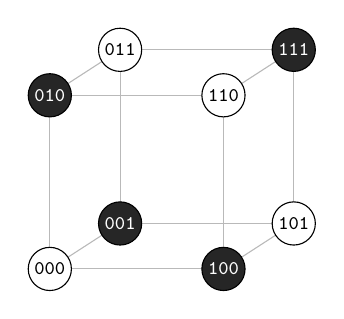
\begin{tikzpicture}[scale=1.05,
  ctr/.style={circle, draw, fill=black!85, text=white, inner sep=1.4pt,
              font=\scriptsize\ttfamily},
  non/.style={circle, draw, fill=white, inner sep=1.4pt,
              font=\scriptsize\ttfamily},
  ed/.style={gray!55}]
  % cube coordinates: back face offset
  \def\dx{0.85}\def\dy{0.55}
  \coordinate (c000) at (0,0);
  \coordinate (c100) at (2.1,0);
  \coordinate (c010) at (0,2.1);
  \coordinate (c110) at (2.1,2.1);
  \coordinate (c001) at (\dx,\dy);
  \coordinate (c101) at (2.1+\dx,\dy);
  \coordinate (c011) at (\dx,2.1+\dy);
  \coordinate (c111) at (2.1+\dx,2.1+\dy);
  \foreach \a/\b in {c000/c100, c000/c010, c100/c110, c010/c110,
                     c001/c101, c001/c011, c101/c111, c011/c111,
                     c000/c001, c100/c101, c010/c011, c110/c111}
    \draw[ed] (\a) -- (\b);
  \node[non] at (c000) {000};
  \node[ctr] at (c100) {100};
  \node[ctr] at (c010) {010};
  \node[non] at (c110) {110};
  \node[ctr] at (c001) {001};
  \node[non] at (c101) {101};
  \node[non] at (c011) {011};
  \node[ctr] at (c111) {111};
\end{tikzpicture}
\caption{$\Kflat(3) = \gtwo(Q_3) = 4$. Filled vertices are the record's four
centres---the odd-weight parity class. Every non-centre has all three of its
neighbours in $C$, so $\dmin = 3$ and the margin is $2/3$.}
\label{fig:q3}
\end{figure}

\subsection{Reproducing every number in this paper}
\label{app:repro}

\begin{verbatim}
python run.py verify   # integrity, then the checks
python run.py audit    # printed numbers vs artifacts
python run.py score    # pre-registered predictions
python run.py figures  # regenerate every figure

# the only step needing a solver, run once:
python src/make_certificates.py
\end{verbatim}

\noindent
\texttt{verify\_all.py} is an independent reimplementation: it rebuilds
$\gtwo(\Qn)$ for $n \le 4$ by complete enumeration of all $2^{2^n}$ subsets,
rechecks every certified code for $2$-domination from scratch, constructs the
record of Lemma~\ref{lem:gen-margin} explicitly and evaluates its distortion and
its all-teammate-profile margin by direct enumeration, re-derives the shell
exclusions, compares the one-bit record against the closed form of
Theorem~\ref{thm:onebit}, and checks every step of
Proposition~\ref{prop:antipodal}---the Rademacher identity and its monotonicity,
the bound \eqref{eq:LB} over all $4^n$ reconstruction pairs at $n = 3,5$ and over
all $(p,m)$ orbits at $n = 7,9$, and feasibility of $r^\ast$. It recomputes every
cell of Table~\ref{tab:ratio} from the two bounds on $\gtwo(\Qn)$, and it checks
the counterexamples of Section~\ref{sec:threshold} by direct enumeration: at
$n = 3,4$ under the Bernoulli$(0.7)$ prior it enumerates every $K$-subset,
identifies the $\pi$-optimal codes, and exhibits a flat record with
$D = \Dnull(K)$ and $\gamma > 0$ at a $K$ below the withdrawn threshold. All $99$ checks pass in the pinned environment (Python 3.10.11, NumPy 2.2.6, SciPy
1.15.3).

\paragraph{A correction, and what it says about our verification.}
An earlier version of this paper claimed a general-prior threshold of
$2^n - (n-1)$. It was wrong, and the way it was wrong is worth recording. Both
verification routes---the solver-free checks and the independent
\texttt{prior\_threshold.py} MILP---searched for a \emph{2-dominating} set, so
both encoded the same incorrect reading of Lemma~\ref{lem:necessity}. They
agreed on $6$, $28$ and $122$ at $n = 3,5,7$, and their agreement was worth
nothing, because independence of implementation does not buy independence of
specification. The error was caught by a test that asked a different
question---relax $\gamma$ and ask an LP directly whether $\Dnull(K)$ is
attainable---rather than by a second implementation of the same question.

The MILP-derived facts---infeasibility of $2$-domination at $(n,K) = (5,9)$,
$(7,29)$, $(7,30)$, $(7,31)$, $(9,94)$, $(9,95)$ and $(9,96)$---are the only
claims that require a solver, and each is a proved-infeasible status rather than
a time limit. Infeasibility admits no small witness, so these are the only claims
the solver-free verifier cannot recheck; the $n=9$ rows were re-proved in the
pinned environment by \texttt{gamma2\_n9\_lb\_rerun.py}.

\paragraph{Theorem~\ref{thm:prior}, machine-checked.}
The three load-bearing claims---the edge structure of
Lemma~\ref{lem:edge-structure}, the strict descent of
Lemma~\ref{lem:strict-descent}, and the closed form of
Lemma~\ref{lem:gen-margin} against the Theorem~\ref{thm:elim} LP---were checked
on all $47{,}017$ $\pi$-optimal codes at $n \le 4$ over eight product priors, by
exhaustive search over \emph{every} code at $n = 3,4$ and over every
radius-$\ge 2$ configuration at $n = 5$ (vertex-transitivity and coordinate
permutation place the bad edge at $(0^n, e_1)$, reducing $2^{32}$ codes to
$724{,}566$), and on $20{,}000$ random codes at $n \le 7$, of which $8{,}517$
satisfy the hypothesis of Lemma~\ref{lem:strict-descent} and all $8{,}517$
satisfy its conclusion. No violation of any kind was found. We note that the
first run of this check \emph{failed}, correctly: an earlier draft of
Lemma~\ref{lem:edge-structure} applied fixed-centre parity to the distance to the
\emph{set}, and the harness rejected it at $n=3$, $K=2$ rather than passing
silently.

\paragraph{The registered predictions, counted.}
$22$ predictions were registered and hashed before each harness was written. $5$
were registered as derivations---predictions whose failure would mean a theorem
or the code was wrong. One of those, that a sampled run reproduces the exact
enumeration, we re-graded to uncertain \emph{before} scoring, because convergence
of an empirical encoder is a statistical claim and not a derivation; that leaves
$4$, and all $4$ held. Of the remaining $18$, $10$ were falsified, $7$ were
confirmed, and $1$ was not scoreable because it referred to a task design we
replaced before running it. Every falsification is reported as a falsification,
here and in the sections above.

\section{Mechanisms, in full}
\label{app:mechdetail}

Everything above describes records chosen \emph{optimally}. No coordinator
chooses a record that way. It keeps a count, or a threshold, or the first few
sub-agents' reports, or hashes the episode into a fixed number of buckets --- and
it does so through a noisy view of what each agent actually did. This section
evaluates those mechanisms, none of which was designed to be optimal, and asks
where they land.

\paragraph{Setup.}
Every profile is enumerated, so the numbers are exact and there is no sampling,
no seed and no error bar. For each mechanism we measure the Bayes reconstruction
error $D$ and the largest all-teammate-profile margin $\gamma$ any bounded
payment rule can extract. The margin is computed \emph{via
Theorem~\ref{thm:elim}}: one LP per agent, rather than a search over payment
rules. The experiment therefore uses the paper's main tool as its instrument.
Under noise, agent~$i$'s effort is observed as $X_i$ with
$\Pr[X_i \ne S_i] = \eta$; the mechanism sees $X$ while reconstruction and
payment are still judged against the true $S$.

Predictions were written down and hashed before the harness was written; two of
them turned out to be wrong, and we report both.

\begin{table}[t]
\centering
\caption{Compaction mechanisms at $n = 5$, uniform prior, no noise. ``Flat''
means $D = \Dnull(K)$ \emph{and} $\gamma > 0$. The last two rows are the same
size and the same distortion.}
\label{tab:mechanisms}
\small
\begin{tabular}{@{}lrrrrl@{}}
\toprule
mechanism & $K$ & $D$ & $\Dnull(K)$ & $\gamma$ & flat \\
\midrule
full        & $32$ & $0.0000$ & $0.0000$ & $1.0000$ & yes \\
count       & $6$  & $1.5625$ & $0.8750$ & $0.2000$ & no \\
threshold   & $2$  & $1.5625$ & $1.5625$ & $0.0000$ & no \\
prefix-4    & $16$ & $0.5000$ & $0.5000$ & $0.0000$ & no \\
prefix-2    & $4$  & $1.5000$ & $1.1250$ & $0.0000$ & no \\
top-2       & $16$ & $0.7188$ & $0.5000$ & $0.0000$ & no \\
hash-10     & $10$ & $1.5000$ & $0.6875$ & $0.0000$ & no \\
\midrule
flat        & $10$ & $0.6875$ & $0.6875$ & $0.5000$ & \textbf{yes} \\
kmedian     & $10$ & $0.6875$ & $0.6875$ & $0.0000$ & no \\
\bottomrule
\end{tabular}
\end{table}

\paragraph{The theory survives contact.}
No mechanism beats the frontier: every one sits on or above $\Dnull(K)$ for its
own $K$, and every two-label mechanism sits on or above the exact frontier of
Theorem~\ref{thm:onebit}. No mechanism below $K = \gtwo(\Qn)$ is flat. These
were derivations rather than guesses --- their failure would have meant a bug or
a false theorem --- but they are checked against records nobody tuned.

\paragraph{The last two rows are the paper.}
At $n = 5$, \texttt{flat} and \texttt{kmedian} use the same ten labels and incur
\emph{the same} distortion $0.6875 = \Dnull(10)$. One admits a payment rule with
margin $1/2$; the other admits none at all, at any price, for any bounded
decoder. Nothing separates them but where the labels were placed. A designer
comparing records on reconstruction quality alone cannot see this difference, and
the same holds at $n = 3$ ($\gamma = 2/3$ against $0$).

\paragraph{Aggregates fail, but not where we predicted.}
We expected \texttt{count} --- ``how many agents succeeded'' --- to have full
margin and poor reconstruction, since one agent's deviation always moves the
count by exactly one. That is what the edge condition
(Corollary~\ref{cor:edge}) suggests. It is wrong. The measured margin is exactly
$1/n$: $0.3333$ at $n=3$, $0.2000$ at $n=5$. The minimax in
Theorem~\ref{thm:elim} is over \emph{mixtures} of teammate profiles, and a
uniform mixture telescopes --- the intermediate shifts cancel and only the two
endpoints survive, leaving $\tfrac{1}{n}$. A point-mass intuition misses this
entirely, which is the clearest illustration we have of why the elimination
theorem is needed rather than its corollary. Aggregates are therefore
\emph{both} margin-poor and reconstruction-poor, and the margin decays with team
size exactly as the label budget argument in Section~\ref{sec:agents} suggests it
should.

\paragraph{A per-agent witness for every agent, or none.}
\texttt{prefix-$m$} retains the first $m$ agents' bits and drops the rest. Its
margin is exactly zero for every $m < n$, at every $n$ tested --- the dropped
agents are invisible, and the margin is a minimum over agents. The design rule is
therefore sharper than ``keep per-agent information'': partial per-agent
retention buys nothing. \texttt{prefix-4} at $n=5$ is the sharpest case, since it
is simultaneously reconstruction-optimal for its budget and worth nothing for
accountability.

\paragraph{Noise, where both our predictions failed.}
We predicted margins would fall continuously with $\eta$. They do not. At
$n = 5$ the margin of \texttt{flat} \emph{rises} from $0.5000$ to $0.5196$ as
$\eta$ goes from $0$ to $0.05$, before falling to $0.4175$ at $\eta = 0.2$. More
strikingly, noise \emph{creates} margin where a deterministic record had none: at
$\eta = 0.1$, \texttt{kmedian} goes from $\gamma = 0$ to $0.1973$ at $n=5$, and
\texttt{threshold} from $0$ to $0.1440$ at $n=3$. The reason is visible once
stated: a deterministic record is insensitive to an agent whose flip does not
change the label, whereas under noise every flip shifts the label
\emph{distribution} a little. Blur can buy accountability.

This does not contradict Section~\ref{sec:threshold}. A record that factors
through the channel is a restricted class of stochastic encoder, so the best it
can achieve is $\Dnull^{\eta}(K) \ge \Dnull(K)$, and we report both baselines
rather than conflating them; no noisy mechanism attains the unrestricted
optimum. The honest reading is that observation noise trades reconstruction for
sensitivity, and that a designer who cannot afford labels may be able to afford
noise instead. We did not anticipate this and do not develop it further here.

\paragraph{The tilted prior, in mechanisms.}
Under a product Bernoulli$(0.7)$ prior the construction built for the uniform
case stops being optimal --- at $n=5$ it incurs $0.7123$ against $\Dnull(10) =
0.3815$ --- and no mechanism at $K = \gtwo(\Qn)$ is flat. This is a statement
about \emph{these} mechanisms, all of which were designed against the uniform
prior; it is not evidence about where the tilted threshold lies, which
Section~\ref{sec:threshold} leaves open.


\begin{figure}[t]
\centering
% Generated by make_figures2.py -- do not edit by hand.
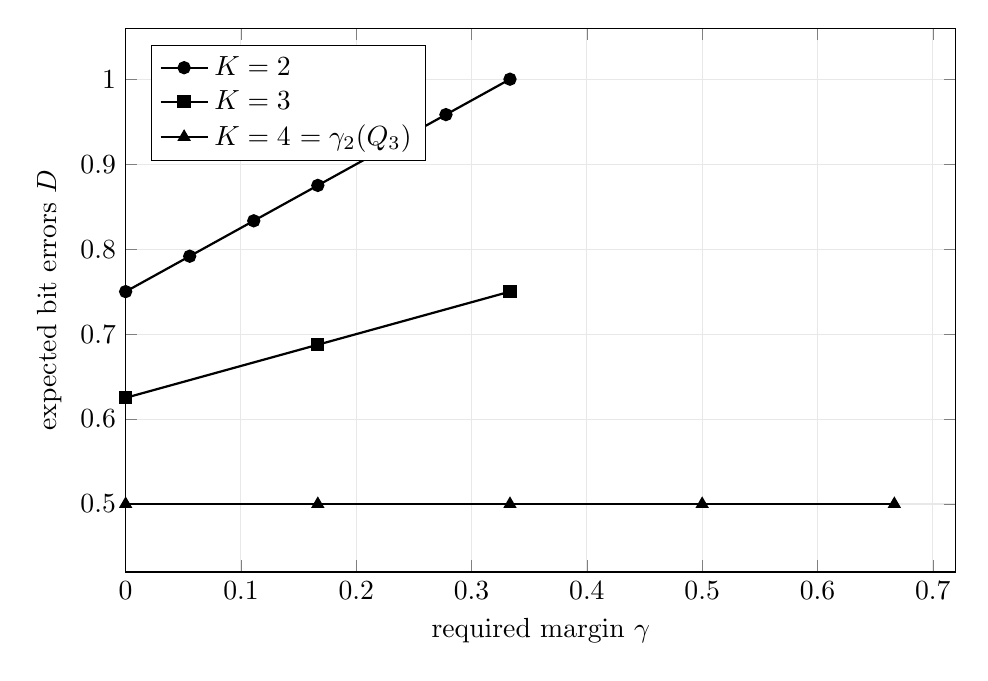
\begin{tikzpicture}
\begin{axis}[
  width=\columnwidth, height=0.70\columnwidth,
  xlabel={required margin $\gamma$},
  ylabel={expected bit errors $D$},
  xmin=0, xmax=0.72, ymin=0.42, ymax=1.06,
  legend pos=north west, legend cell align=left,
  grid=major, grid style={gray!18},
]
\addplot[thick, mark=*] coordinates {(0.000000,0.750000) (0.055556,0.791667) (0.111111,0.833333) (0.166667,0.875000) (0.222222,0.916667) (0.277778,0.958333) (0.333333,1.000000)};
\addlegendentry{$K=2$}
\addplot[thick, mark=square*] coordinates {(0.000000,0.625000) (0.166667,0.687500) (0.333333,0.750000)};
\addlegendentry{$K=3$}
\addplot[thick, mark=triangle*] coordinates {(0.000000,0.500000) (0.166667,0.500000) (0.333333,0.500000) (0.500000,0.500000) (0.666667,0.500000)};
\addlegendentry{$K=4$ $=\gamma_2(Q_3)$}
\end{axis}
\end{tikzpicture}

\caption{The tradeoff at intermediate record sizes, $n = 3$. At $K=2$ it is
the exact frontier of Theorem~\ref{thm:onebit}; at $K=3$ it is shallower and
runs out of feasible margin sooner; at $K = 4 = \gtwo(Q_3)$ it is
\emph{flat}---distortion stays at $\Dnull(4)$ all the way to the maximum
margin $1-1/\dmin = 2/3$. Curves are achievability: each point is a record
that exists. They reproduce $\Dnull(K)$ at $\gamma=0$ and Theorem~\ref{thm:onebit} at $K=2$, both asserted in the harness.}
\label{fig:frontierK}
\end{figure}

\begin{figure}[t]
\centering
% point labels overhang the axis box, so scale the whole picture to the column
\resizebox{\columnwidth}{!}{% Generated by make_figures2.py -- do not edit by hand.
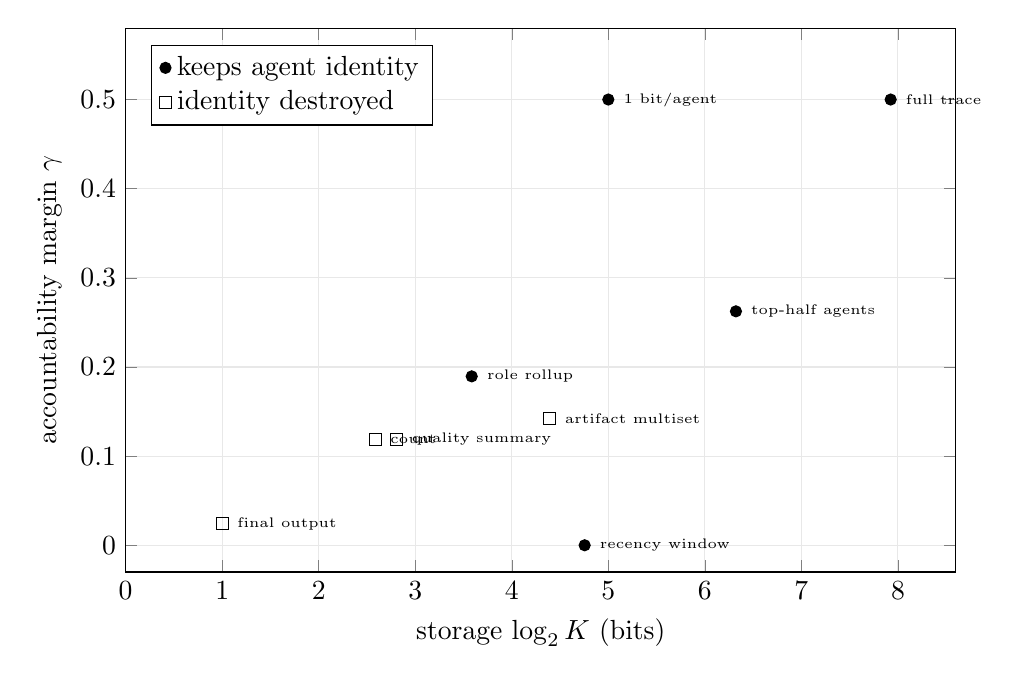
\begin{tikzpicture}
\begin{axis}[
  width=\columnwidth, height=0.70\columnwidth,
  xlabel={storage $\log_2 K$ (bits)},
  ylabel={accountability margin $\gamma$},
  xmin=0, xmax=8.6, ymin=-0.03, ymax=0.58,
  legend pos=north west, legend cell align=left,
  grid=major, grid style={gray!18},
  nodes near coords, point meta=explicit symbolic,
  every node near coord/.append style={font=\tiny, anchor=west, xshift=2pt},
]
\addplot[mark=*, only marks, mark size=2pt] coordinates {(3.5850,0.189474) [role rollup] (4.7549,0.000000) [recency window] (5.0000,0.500000) [1 bit/agent] (6.3219,0.262400) [top-half agents] (7.9248,0.500000) [full trace]};
\addlegendentry{keeps agent identity}
\addplot[mark=square, only marks, mark size=2.2pt] coordinates {(1.0000,0.024300) [final output] (2.5850,0.119020) [count] (2.8074,0.119020) [quality summary] (4.3923,0.142510) [artifact multiset]};
\addlegendentry{identity destroyed}
\end{axis}
\end{tikzpicture}
}
\caption{Storage against accountability for the episode records at $n=5$.
Records that keep agent identity sit high regardless of how few bits they
use; records that keep content but discard authorship sit low regardless of
how many.}
\label{fig:identity}
\end{figure}
\subsection{An episode, not just a profile}
\label{app:episodes}

The experiment above compresses the effort profile itself, which concedes the
abstraction most open to question: that what an agent did can be written as one
bit. So we put an episode in between. A coordinator fans out $n$ subtasks; agent
$i$ has a controlled effort bit $S_i$ and returns an artifact whose quality is
drawn from one of two distributions according to it; the coordinator ships iff at
least half the subtasks completed. A \emph{record} now compresses the trace
$(A_1,\dots,A_n,F)$, so the encoder $\enc(\cdot \mid S)$ of
Section~\ref{sec:model} is \emph{measured} rather than defined. Agents are
conditionally independent given $S$, so it is computed exactly by enumerating
artifact tuples. We also ran $200{,}000$ sampled episodes as a cross-check:
they reproduce the exact values to within $0.025$ at $n \le 5$. At $n = 6,7$
the label space outgrows the episode budget --- the full trace alone has $2187$
labels at $n=7$ against $1562$ episodes per profile --- so the empirical
encoder is too sparse there to estimate a margin, and every number we report is
the exact one.

\begin{table}[t]
\centering
\caption{Records over an episode trace, $n = 5$, exact. ``Content'' is not what
buys accountability: \texttt{global\_summary} keeps every artifact and loses only
\emph{who} produced it.}
\label{tab:episodes}
\small
\begin{tabular}{@{}lrrr@{}}
\toprule
record & $K$ & $D$ & $\gamma$ \\
\midrule
full trace              & $243$ & $1.2500$ & $0.5000$ \\
one bit per agent       & $32$  & $1.2500$ & $0.5000$ \\
top-half agents only    & $80$  & $1.2923$ & $0.2624$ \\
multiset of artifacts   & $21$  & $1.9718$ & $0.1425$ \\
count of completions    & $6$   & $2.0194$ & $0.1190$ \\
final output only       & $2$   & $2.1118$ & $0.0243$ \\
\bottomrule
\end{tabular}
\end{table}

\paragraph{Identity, not volume.}
The ordering of records by margin follows how much \emph{per-agent identity}
survives, not how many bits do. We pre-registered this as a quantitative
claim---that removing identity costs proportionally more margin than it saves
storage---and it holds in every matched-storage comparison at every
$n \in \{3,\dots,7\}$: the ratio of relative margin lost to relative storage
saved never drops below $1.07$, with a median around $1.4$--$2.3$. We also
predicted that ratio would exceed $3$ everywhere and that it would grow with
$n$; both were wrong. The direction is robust and the magnitude is usually
modest, with the striking cases being specific pairs rather than the rule. \texttt{multiset of artifacts} retains every
artifact in full and discards only the association between artifact and author;
it keeps far more of the trace than a single bit per agent, and has less than a
third of the margin. At $n = 3$ it even has \emph{more} labels ($10$ against
$8$) and still less than half the margin. This is the design rule stated as a
measurement: accountability is priced in attribution, not in volume.

\paragraph{One bit per agent is not a compromise.}
At both $n$ tested, \texttt{one bit per agent} matches the \emph{full trace} on
both axes exactly---$D = 1.2500$ and $\gamma = 0.5000$ at $n = 5$, using $32$
labels against $243$. We did not predict this. Under this episode model the
per-agent bit is a sufficient statistic for both jobs, so the $7.6\times$
compression is free in the strong sense: nothing about reconstruction or
accountability is given up.

\paragraph{Where we were wrong again, and what it teaches.}
We predicted that retaining bits for only the top half of agents would give
margin exactly $0$, as fixed truncation does in Table~\ref{tab:mechanisms}. It
does not: it keeps $0.2624$ of the available $0.5000$. The difference is that
\emph{which} agents are retained is itself determined by what they did, so an
agent who shirks changes its own probability of appearing in the record. Selection
that depends on behaviour is far better than selection fixed in advance, which
sharpens the rule from Section~\ref{sec:agents}: a record may drop agents, but not
on a schedule decided before the episode. We also predicted the coordinator's
ship/no-ship bit would be worth nothing; it retains a small margin that decays
quickly in $n$ ($0.0900$ at $n=3$, $0.0243$ at $n=5$).

\input{sections/066b-llm-appendix}
\section{Design implications}
\label{app:design}

The mathematics above answers a question a system designer actually has: given a
budget on what survives an episode, what must be kept so that someone can still
be paid, credited or blamed for their own work. Four rules follow, each traceable
to a specific result rather than to intuition.

\paragraph{R1. Preserve agent identity before preserving content.}
This is the sharpest empirical finding of Section~\ref{app:episodes} and it is
not what a compression-minded engineer expects. The record that keeps every
artifact in full and discards only \emph{who produced each one} retains more of
the trace than a single bit per agent, and has less than a third of the
accountability margin ($0.1425$ against $0.5000$ at $n=5$; at $n = 3$ it has
\emph{more} labels and still less than half the margin). Attribution is what is
being bought, and content is not a substitute for it. The magnitude varies: across
$n = 3,\dots,7$ the cost of removing identity, measured against the storage it
saves, is reliably greater than one but usually between $1.4$ and $2.3$ rather
than the near-sixfold figure that case gives. The direction is the rule; the
size is not.

\paragraph{R2. Keep one witness per agent, for every agent.}
One retained bit per agent is flat with margin $1$: the tension does not exist
there. Under the episode model it is not even a compromise, matching the full
trace on both reconstruction and margin while using $32$ labels instead of $243$
(Table~\ref{tab:episodes}). The important word is \emph{every}: a record that
keeps per-agent bits for a fixed subset and drops the rest has margin exactly
zero, because the margin is a minimum over agents and the dropped ones are
invisible (Table~\ref{tab:mechanisms}). Partial per-agent retention on a schedule
fixed in advance buys nothing at all.

\paragraph{R3. Do not settle from a global count.}
An aggregate such as ``how many subtasks completed'' has accountability margin
exactly $1/n$ --- it decays with the size of the team, which is precisely the
regime where deferred settlement matters most. Note this is weaker than the
single-deviation intuition suggests: one agent always moves the count by one, yet
mixtures of teammate behaviour cancel the intermediate shifts
(Section~\ref{sec:experiment}). Counts are cheap and feel informative; they are
close to worthless for attribution at scale.

\paragraph{R4. More retained content does not mean more accountability.}
The two axes are close to independent, and the paper's central object is a pair
of records that makes this concrete: at $n = 5$ two ten-label records incur
\emph{identical} distortion $\Dnull(10)$, and one supports margin $1/2$ while the
other supports none at any price. A designer comparing candidate records on
reconstruction quality alone---which is the natural thing to measure---cannot
tell them apart. Accountability has to be measured separately, and
Theorem~\ref{thm:elim} makes that measurement cheap: one linear program per
agent, no search over payment rules.

\paragraph{A caveat that cuts the other way.}
Two of these rules are robustness claims, and Section~\ref{sec:experiment} found
one boundary. Selection that \emph{depends on what agents did} is much better
than selection fixed in advance: retaining bits for the top half of agents by
observed quality keeps $0.2624$ of the available $0.5000$, not the zero that R2's
fixed-subset case gives, because an agent who shirks changes its own probability
of being recorded. If a budget forces dropping agents, drop them on the basis of
the episode rather than on a schedule.


\end{document}
